\chapter{Optical waveguides}
\section{Geometrical-optics description}
\subsection{Step-index (SI) waveguides}
	\begin{wrapfigure}[7]{l}{6cm}
	\vspace{-5mm}
	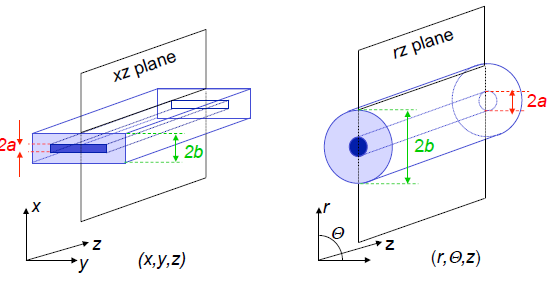
\includegraphics[scale=0.4]{ch1/image1}
	\captionof{figure}{ }
	\end{wrapfigure}
Dans un premier temps, on va seulement considérer la cas à deux dimensions : 
la lumière se propage dans un plan ($xy$ pour les guides plans, $rz$ pour les cylindriques). 
Pour l'instant, considérons $b$ comme étant infini. Généralement, le cœur mesure 9-10 microns
alors que la gaine est de 125 microns (vient ensuite le coating pour éviter les microcourbures).\\

	\begin{wrapfigure}[11]{r}{7cm}
	\vspace{-9mm}
	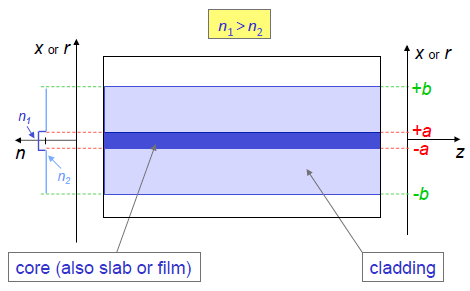
\includegraphics[scale=0.6]{ch1/image2}
	\captionof{figure}{ }
	\end{wrapfigure}
Effectuons une coupe dans le plan $rz$ de la fibre. En optique géométrique, il faut que la dimension physique dans laquelle la lumière se propage soit plus grand que la longueur d'onde. Autrement dit
\begin{equation}
\lambda \ll a,b
\end{equation}
Ceci est nécessaire afin de pouvoir modéliser la propagation par des rayons. Nous faisons l'hypothèse
que le cœur et la gaine sont des diélectriques homogènes\footnote{Utiliser un conducteur n'a pas de sens
: mouvement des charges libres, effets joule, \dots} où l'on suppose $n_1>n_2$, les indices de
réfractions du cœur et de la gaine. Nous verrons plus tard qu'il s'agit en fait d'une condition
nécessaire. Nous ferons aussi l'hypothèse d'un milieu sans pertes et invariant pour une translation
selon $z$ (pas de courbures).\\

La loi de Snell-Descartes exprime le changement de direction d'un faisceau lors de la traversée
d'une paroi. Chaque milieu à une capacité à "ralentir" la lumière, caractérisé par son indice
de réfraction $n\equiv c/v$
\begin{equation}
n_1 \sin\theta_1=n_2 \sin\theta_2
\end{equation}
Si $n_1>n_2$, le faisceau réfracté se rapproche plus rapidement du dioptre : le rayon est élevé alors
que dans le cas contraire, il est "rabattu". Dans le premier cas, le rayon peut remonter jusqu'à
l'horizontale $(\pi/2)$. Au dessus de cet angle, il sera totalement réfléchi : c'est le phénomène
de réflexion totale\footnote{Pour l'histoire, ceci explique pourquoi un diamant ne brille pas dans
l'eau.}\\


	\begin{wrapfigure}[9]{r}{7.5cm}
	\vspace{-9mm}
	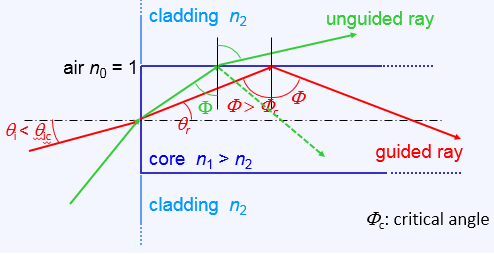
\includegraphics[scale=0.6]{ch1/image3}
	\captionof{figure}{ }
	\end{wrapfigure}
Considérons le rayon vert ci-contre. Initialement dans l'air, il rencontre l'interface air-verre ($
n_1$) ou il y a des réflexions. Ensuite, il rencontre l'interface cœur-gaine où on observe un 
phénomène de réflexion partielle et de réfraction. Il est possible d'avoir une \textbf{réflexion
totale} si le rayon a une incidence assez rasante et si $n_1>n_2$.\\

Regardons le cas particulier d'un angle critique (rouge). En appliquant la loi de S-D, on trouve
\begin{equation}
\left.\begin{array}{ll}
{n_0}\sin {\theta _i} &= {n_1}\sin {\theta _r}\\
{n_0}\sin {\theta _{ic}} &= \sin {\theta _{ic}} = {n_1}\sin {\theta _{rc}} = {n_1}\cos {\Phi _c}\\
{n_1}\sin {\Phi _c} &= {n_2}\sin \frac{\pi }{2} = {n_2}
\end{array}\right\}\cos {\Phi _c} = \sqrt {1 - {{\sin }^2}{\Phi _c}} = \sqrt {1 - {{\left( {{{{n_2}} \mathord{\left/
 {\vphantom {{{n_2}} {{n_1}}}} \right.
 \kern-\nulldelimiterspace} {{n_1}}}} \right)}^2}}
\end{equation}
où la première ligne correspond à l'interface air-cœur et la dernière au cas de réflexion totale. On 
peut ainsi trouver une expression pour l'angle critique. \\

\cadre{Le rayon sera guidé si\begin{equation}
\Phi  > {\Phi _c}
\end{equation}}\ \\

\begin{wrapfigure}[6]{l}{7.5cm}
	\vspace{-5mm}
	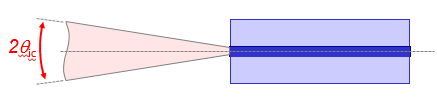
\includegraphics[scale=0.6]{ch1/image4}
	\captionof{figure}{ }
	\end{wrapfigure}
L'\textbf{ouverture numérique} renseigne le "cône d'acceptance" des rayons, afin que ceux-ci soient
guidés. Par définition
\begin{equation}
NA \buildrel \Delta \over = {n_0}\sin {\theta _{ic}} = {n_1}\sqrt {1 - {{\left( {{{{n_2}} \mathord{\left/
 {\vphantom {{{n_2}} {{n_1}}}} \right.
 \kern-\nulldelimiterspace} {{n_1}}}} \right)}^2}}  = \sqrt {{n_1}^2 - {n_2}^2} 
\end{equation}
Souvent on retrouve cette information dans les data-sheet pas pas $n_1$ et $n_2$, car l'AN est plus
facile à mesurer. On utilise souvent l'\textbf{indice de réfraction normalisé} $\Delta n \buildrel \Delta \over = {{\left( {{n_1} - {n_2}} \right)} \mathord{\left/
 {\vphantom {{\left( {{n_1} - {n_2}} \right)} {{n_1}}}} \right.
 \kern-\nulldelimiterspace} {{n_1}}}$ ainsi que l'indice de réfraction moyen $\bar n \buildrel \Delta \over = {{\left( {{n_1} + {n_2}} \right)} \mathord{\left/
 {\vphantom {{\left( {{n_1} + {n_2}} \right)} 2}} \right.
 \kern-\nulldelimiterspace} 2}$.\\
 
En pratique, on rencontre souvent un guidage dit faible : l'angle d'incidence est très proche de 
$90^\circ $ et on dit alors que $n_1\approx n_2$. Plus l'AN est grande, plus la propagation sera rapide. Un ordre de grandeur usuel pour celle-ci est de 0.2.

\subsubsection{Multipath dispersion (or Modal dispersion)}

\begin{wrapfigure}[8]{r}{4.5cm}
	\vspace{-5mm}
	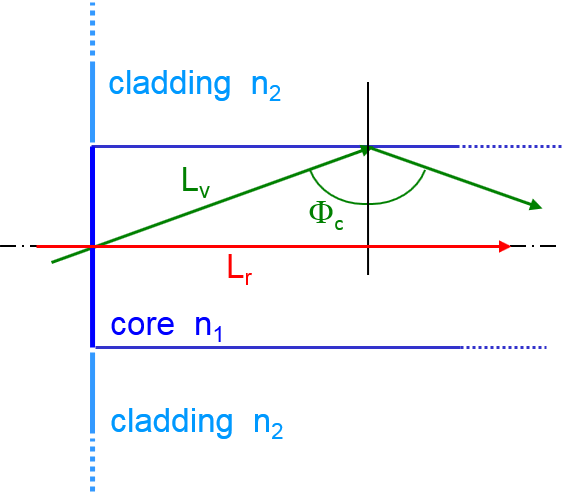
\includegraphics[scale=0.34]{ch1/image5}
	\captionof{figure}{ }
	\end{wrapfigure}
Le problème c'est qu'un rayon qui se propage sur l'axe ne va pas faire le même parcours que 
celui qui fait des zigzag. La vitesse de groupe est la même, mais il y aura un délai associé 
à cette différence de chemin entre les deux. Pour calculer ce délai, on s'intéresse à la différence
de chemin $\delta l$ entre les deux rayons (rouge et vert) à l'aide d'un joli triangle rectangle
\begin{equation}
\delta l = {L_v} - {L_r} = {L_r}\left( {{1 \mathord{\left/
 {\vphantom {1 {\sin {\Phi _c}}}} \right.
 \kern-\nulldelimiterspace} {\sin {\Phi _c}}}} \right) - {L_r} = {L_r}\left[ {\left( {{{{n_1}} \mathord{\left/
 {\vphantom {{{n_1}} {{n_2}}}} \right.
 \kern-\nulldelimiterspace} {{n_2}}}} \right) - 1} \right]
\end{equation}
Il faut ensuite sommer ceci sur la longueur $L$ de la fibre 
\begin{equation}
\Delta L = \sum {\delta l}  = L\left[ {\left( {{{{n_1}} \mathord{\left/
{\vphantom {{{n_1}} {{n_2}}}} \right.
\kern-\nulldelimiterspace} {{n_2}}}} \right) - 1} \right]
\end{equation}
En supposant que la vitesse de phase $(c/n)$ vaut à peu près la vitesse de groupe, on trouve
\begin{equation}
\Delta t = \frac{{\Delta L}}{{{c \mathord{\left/
 {\vphantom {c {{n_1}}}} \right.
 \kern-\nulldelimiterspace} {{n_1}}}}} = \frac{L}{c}{n_1}\left[ {{{\left( {{n_1} - {n_2}} \right)} \mathord{\left/
 {\vphantom {{\left( {{n_1} - {n_2}} \right)} {{n_2}}}} \right.
 \kern-\nulldelimiterspace} {{n_2}}}} \right] = \frac{L}{c}{n_1}\left[ {{{\left( {{n_1}\Delta n} \right)} \mathord{\left/
 {\vphantom {{\left( {{n_1}\Delta n} \right)} {{n_2}}}} \right.
 \kern-\nulldelimiterspace} {{n_2}}}} \right]
\end{equation}
où encore
\begin{equation}
\Delta t = \frac{L}{c}\Delta n\frac{{{n_1}^2}}{{{n_2}}}
\end{equation}
Une grande AN ($\propto \sqrt{\Delta n})$ facilité l'injection dans la lumière, mais un grand $\Delta t$ $(\propto\Delta n)$ limite le taux de bit.

\begin{center}
	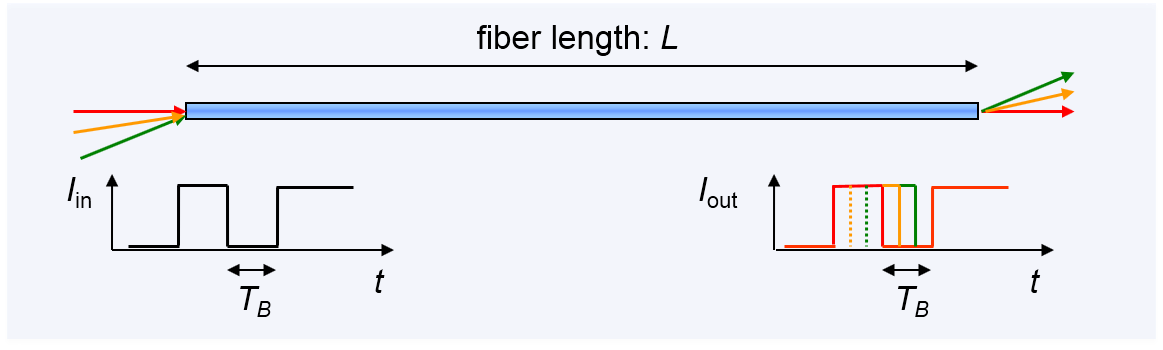
\includegraphics[scale=0.4]{ch1/image6}
	\captionof{figure}{ }
\end{center}

S'il y a une différence de vitesse de groupe, l'information va avoir tendance à s'étaler dans le 
temps. Les flancs vont alors s'étaler et il ne sera plus disponible de distinguer 0 et 1. Il faut que
cette dispersion temporelle soit inférieure au temps d'un bit : $\Delta t < T_B = 1/B$. Dès lors, 
$B\Delta t < 1 \Leftrightarrow B\frac{L}{c}{n_1}\left[ {{{\left( {{n_1}\Delta n} \right)} \mathord{\left/
 {\vphantom {{\left( {{n_1}\Delta n} \right)} {{n_2}}}} \right.
 \kern-\nulldelimiterspace} {{n_2}}}} \right] < 1$. On en tire (sous l'hypothèse que la taille du 
 cœur est grande par rapport à $\lambda$\\
 
 \cadre{\begin{equation}
 BL < \frac{c}{{\Delta n}}\frac{{{n_2}}}{{n_1^2}}
 \end{equation}}\ \\
 
Le produit $BL$ est donc bien un paramètre important pour une fibre. Celui-ci nous informe qu'un
signal de 200Mbits/s ne peut être transmis que sur une distance de 100m pour une fibre Si multimode. 

\newpage
\subsection{Graded-index (GI) fibers}
Pour réduire le délai entre les rayons guidés, on peut utiliser des fibres à \textbf{gradient} 
d'indice. L'indice change dans le cœur : élevé au centre (ralenti les rayons) et diminue ensuite 
(ralentis un peu moins les rayons)\footnote{Voir notes slides 10 et 11 pour plus de détails.}. 

\begin{center}
	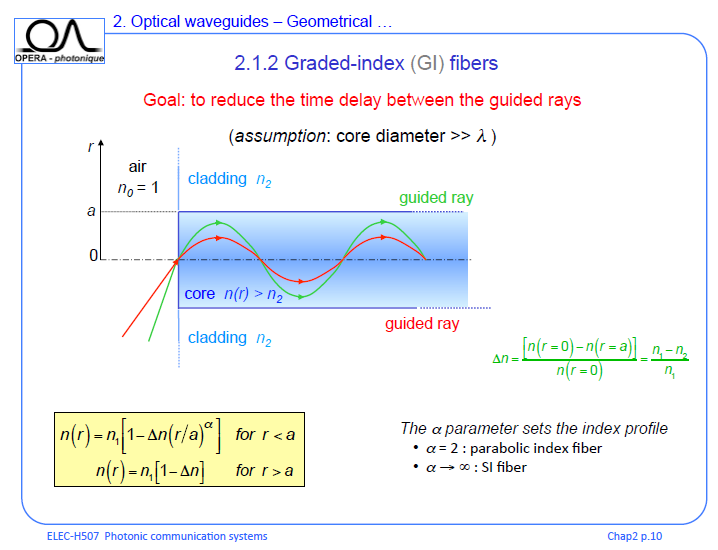
\includegraphics[scale=0.5]{ch1/image8}
	\captionof{figure}{ }
\end{center}

\begin{center}
	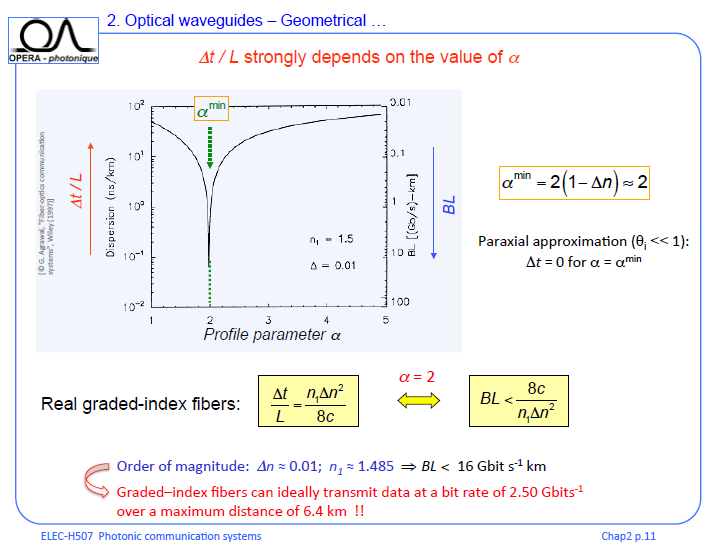
\includegraphics[scale=0.5]{ch1/image9}
	\captionof{figure}{ }
\end{center}


\subsubsection{Limitations of the simple two-dimensional geometrical optics description:}

\begin{wrapfigure}[5]{r}{8cm}
	\vspace{-5mm}
	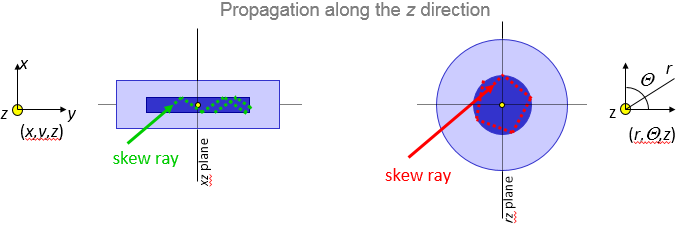
\includegraphics[scale=0.45]{ch1/image7}
	\captionof{figure}{ }
	\end{wrapfigure}
Jusqu'ici nous avons considérer que les rayons se situent uniquement dans des plans $xz/rz$. Or, 
certains rayons peuvent être obliques, hélicoïdaux, \dots\ De plus, que se passe-t-il si le 
cœur a une dimension proche de la longueur d'onde ? Il faut une approche EM!

\section{Electromagnetic analysis – Fields and modes}
\subsection{Step-index planar waveguides}

\begin{wrapfigure}[8]{r}{7cm}
	\vspace{-5mm}
	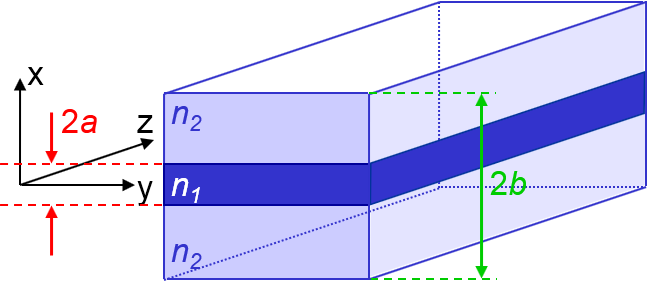
\includegraphics[scale=0.4]{ch1/image10}
	\captionof{figure}{ }
	\end{wrapfigure}
Nous allons commencer par le cas d'un guide d'onde plan. L'idée est de résoudre les équations de 
Maxwell afin de trouver une solution qui satisfait aux conditions limites, continuité, \dots\ soit 
un problème aux valeurs propres d'un certain opérateur différentiel (le propagateur) agissant sur un 
champ.\\

Nous allons faire plusieurs hypothèses
\begin{enumerate}
\item Matériau simple : diélectrique, non magnétique, linéaire, isotropique et sans perte. En gros,
juste $n_1$ et $n_2$ à prendre en compte.
\item Homogène : toujours $n_1$ dans le cœur et $n_2$ dans la gaine
\item Symétrique en $x$ et indépendant en $y,z$ : même matériau pour les deux gaines.
\item La dimension de la gaine ($2b$) est très grande par rapport à celle du cœur ($2a$) : on ne doit
pas se préoccuper de l'interface gaine-coatting.
\end{enumerate}\ 

Nous n'avons ici fait \textbf{aucune} hypothèse sur la taille du cœur, contrairement à l'approche
géométrique. Il peut être très petit ou très grand mais en pratique, il vaut typiquement, $2a \leq 50\
 \mu$m.\\
 

Le point de départ est bien évidemment les équations de Maxwell. Pour un diélectrique non magnétique
\begin{equation}
\nabla  \times \vec{E} =  - \frac{{\partial  \vec{B}}}{{\partial t}},\qquad
\nabla  \times \vec{H} = \frac{{\partial \vec{D}}}{{\partial t}}, \qquad
\nabla .\vec{D} = 0,\qquad
\nabla .\vec{B} = 0
\end{equation} 
L'interaction entre la champ EM et le diélectrique trouve son origine dans le champ de densité de 
polarisation $\vec{P}$ qui prend en compte l'indice de réfraction est les pertes. La polarisation 
doit être non nulle, sans quoi on décrirait le vide.
\begin{equation}
\vec B = \mu_0\vec{H},\qquad\qquad\qquad \vec{D} = \epsilon_0\vec{E}+\vec{P}
\end{equation}
Le champ de densité de polarisation s'obtient par la convolution entre le champ $\vec{E}$ et la
\textbf{susceptibilité électrique}
\begin{equation}
\vec{P}\left( {{\bf{r}},t} \right) = {\varepsilon _0}\int_{ - \infty }^{ + \infty } {\chi \left( {{\bf{r}},t - t'} \right)}  \vdots \vec{E}\left( {{\bf{r}},t'} \right)dt'
\end{equation}
Le système sera ainsi linéaire en $\vec{E}$ et permanent. La susceptibilité est en réalité un 
tenseur de second rang. Heureusement la fibre ne présente pas de biréfringeance (le verre étant 
amorphe, cette hypothèse est bien vérifiée), elle est même isotrope : la susceptibilité se ramène 
à un scalaire. Notons que notre système est bien causal. La convolution temporelle se traite plus
facilement dans le domaine fréquentiel. De plus, le système étant linéaire, il suffira de sommer 
sur toutes les fréquences. On définit la transformée de Fourier avec la convention suivante\footnote{En optique, on utilise souvent $-i\omega t$ alors qu'en électronique on voit $+j\omega t$. Cela ne change rien, il suffit de changer $j\to -i$.}
\begin{equation}
\vec{E}\left( {{\bf{r}},t} \right) = \int_{ - \infty }^{ + \infty } {\vec{\tilde E}\left( {{\bf{r}},\omega } \right)\exp (j\omega t)d\omega } 
\end{equation}
Le champ électrique étant réel, on ne considèrera que les $\omega >0$
\begin{equation}
\vec{E}{\rm{(}}t{\rm{)}} = \vec{A}{\rm{(}}t{\rm{)cos(}}{\omega _0}t + \varphi {\rm{(}}t{\rm{))}}
 = \frac{1}{2}\vec{A}{\rm{(}}t{\rm{)[}}{{\rm{e}}^{j{\rm{(}}{\omega _0}t + \varphi {\rm{(}}t{\rm{))}}}} + c.c{\rm{]}} = \frac{1}{2}{\rm{[}}E{\rm{(}}t{\rm{)}} + {E^*}{\rm{(}}t{\rm{)]}}
\end{equation}
On utilisera $E(t)$ pour décrire le champ électrique et $\vec{E}{\rm{(}}t{\rm{)}} = Re{\rm{[}}E{\rm{(}}t{\rm{)]}}$. On en tire
\begin{equation}
\tilde P\left( {r,\omega } \right) = {\varepsilon _0}\tilde \chi \left( {r,\omega } \right)\tilde E\left( {r,\omega } \right)
\end{equation}
Le terme de l'équation de Maxwell
\begin{equation}
\nabla  \times \nabla  \times \vec{E} =  - \frac{1}{{{c^2}}}\frac{{{\partial ^2}\vec{E}}}{{\partial {t^2}}} - {\mu _0}\frac{{{\partial ^2}\vec{P}}}{{\partial {t^2}}}
\end{equation}
S'écrit alors, dans le domaine fréquentiel
\begin{equation}
\nabla  \times \nabla  \times \tilde E = \left( {1 + \tilde \chi } \right)\frac{{{\omega ^2}}}{{{c^2}}}\tilde E = \kappa \left( {r,\omega } \right)\frac{{{\omega ^2}}}{{{c^2}}}\tilde E
\end{equation}


\begin{wrapfigure}[8]{r}{5cm}
	\vspace{-5mm}
	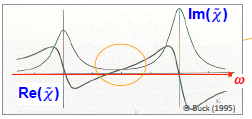
\includegraphics[scale=0.8]{ch1/image11}
	\captionof{figure}{ }
	\end{wrapfigure}
où l'on a introduit la \textbf{constante diélectrique}
\begin{equation}
\kappa \left( {r,\omega } \right) = 1 + \tilde \chi \left( {r,\omega } \right) = {(n - j\alpha c/2\omega )^2} \approx {n^2}
\end{equation}
L'atténuation étant négligeable, $\kappa$ sera réel. Le milieu étant homogène dans le
cœur et la gaine
\begin{equation}
\nabla  \times \nabla  \times {\bf{\tilde E}} = \nabla \left( {\nabla  \cdot {\bf{\tilde E}}} \right) - \Delta {\bf{\tilde E}} =  - \Delta {\bf{\tilde E}}
\end{equation}
Notons que $\kappa$ sera différent dans le cœur et dans la gaine. On trouve alors six équations (identiques pour $\tilde{H}$) équations\\

\cadre{\textsc{Equation d'Helmotz}\begin{equation}
\Delta {\bf{\tilde E}} + \kappa \left( \omega  \right)\frac{{{\omega ^2}}}{{{c^2}}}{\bf{\tilde E}} = 0\qquad\qquad\qquad
\Delta \tilde H + \kappa \left( \omega  \right)\frac{{{\omega ^2}}}{{{c^2}}}\tilde H = 0
\end{equation}
où $\kappa_{core}\neq\kappa_{cladding}$ où la constante diélectrique dépend de la fréquence et où
\begin{equation}
{\kappa _j}\left( \omega  \right)\frac{{{\omega ^2}}}{{{c^2}}} = {n_j}^2\left( \omega  \right)\frac{{{\omega ^2}}}{{{c^2}}} = {n_j}^2\left( \omega  \right){\left( {\frac{{2\pi }}{{{\lambda _0}}}} \right)^2} = {n_j}^2\left( \omega  \right)k_0^2
\end{equation}
avec $j=1$ pour le cœur et $j=2$ pour la gaine.}\ \\

Nous avons donc six équations couplées. Heureusement, seulement deux sont indépendantes : il ne 
faudra résoudre que ces deux-là
\begin{equation}
{\tilde E_y} = {\tilde E_y}({\tilde E_x},{\tilde H_x})\qquad\qquad
{\tilde H_y} = {\tilde H_y}({\tilde E_x},{\tilde H_x})\qquad\qquad
{\tilde E_z} = {\tilde E_z}({\tilde E_x},{\tilde H_x})\qquad\qquad
{\tilde H_z} = {\tilde H_z}({\tilde E_x},{\tilde H_x})
\end{equation}

Le schéma de résolution sera alors le suivant
\begin{enumerate}
\item Tenir compte des symétries de la structure en $(x,y,z)$
\item Séparer le problème pour chaque milieu homogène (cœur et gaine)
\item Appliquer les CL aux interfaces cœur-gaine pour trouver les modes guidés.
\begin{itemize}
\item[$\bullet$] Il faut aussi avoir la continuité des composantes tangentielle de $\vec{E}$ et 
$\vec{E}$ ainsi que les composantes normales de $\vec{B}$ et $\vec{D}$.
\end{itemize}
\item Construire la solution générale (équation linéaire)
\end{enumerate}\ 

La solution générale d'un champ EM dans un guide d'onde est la suivante (idem pour $\tilde{H}$)
\begin{equation}
\tilde E(x,y,z,\omega ) = \sum\limits_m {\left[ {{a_m}{{\tilde E}_m}(x,y,z,\omega ) + {a_{ - m}}{{\tilde E}_{ - m}}(x,y,z,\omega )} \right] + {{\tilde E}_{{\rm{rad}}}}(x,y,z,\omega )} 
\end{equation}
où le premier terme sont les modes progressif, la second les régressif et le dernier, le champ 
radiés (négligeable). 

\subsubsection{Étape 1 : Symétries}
Basé sur les symétries, nous allons chercher par la méthode de séparation des variables une solution
de la forme
\begin{equation}
{E_x}(x,y,z,t) = {\tilde E_x}(x,y,z,\omega )\exp (j\omega t) = {E_x}(x).Y(y).Z(z).\exp (j\omega t)
\end{equation}
et de même pour $H_x$. Nous pouvons procéder à une telle résolution par symétrie de translation en $y,
z$ et dans le temps. Si nous avions un guide plan rectangulaire entouré d'une gaine optique, nous
aurions une seule fonction en $z$, une en $t$ mais également une en $x$ et $y$ ! \\

Nous avons donc
\begin{equation}
\frac{1}{{{{\rm{E}}_x}}}\frac{{{d^2}{{\rm{E}}_x}}}{{d{x^2}}} + \frac{{{\omega ^2}}}{{{c^2}}}\kappa (\omega ,x) + \frac{1}{{\rm{Y}}}\frac{{{d^2}Y}}{{d{y^2}}} + \frac{1}{{\rm{Z}}}\frac{{{d^2}Z}}{{d{z^2}}} = 0
\end{equation}
En $Y$ et $Z$, nous pouvons avoir des solutions exponentielles, sinus, cosinus, sinh et cosh. Il faut
comprendre l'invariance en translation en terme de densité de photon. Comme celui-ci contient un 
module carré, il faut choisir la solution en exponentielles imaginaires. Ceci signifie que les 
"constantes" que vaut ces termes doit être négative. On en tire pour $Y$
\begin{equation}
\frac{1}{{\rm{Y}}}\frac{{{d^2}Y}}{{d{y^2}}} =  - {\gamma ^2}\qquad\qquad\Rightarrow\qquad\qquad
{\rm{Y(}}y{\rm{)}} = {e^{ - j\gamma y}}
\end{equation}
où $\gamma\in\mathbb{R}$. Pour $Z$
\begin{equation}
\frac{1}{{\rm{Z}}}\frac{{{d^2}Z}}{{d{z^2}}} =  - {\beta ^2} \qquad\qquad\Rightarrow\qquad\qquad
{\rm{Z(}}z{\rm{)}} = {e^{ - j\beta z}}
\end{equation}
où $\beta\in\mathbb{R}$. L'équation à résoudre devient alors
\begin{equation}
\frac{{{d^2}{{\rm{E}}_x}}}{{d{x^2}}} + \left[ {\frac{{{\omega ^2}}}{{{c^2}}}\kappa (\omega ,x) - {\beta ^2} - {\gamma ^2}} \right]{{\rm{E}}_x} = 0\qquad\qquad
\frac{{{d^2}{{\rm{H}}_x}}}{{d{x^2}}} + \left[ {\frac{{{\omega ^2}}}{{{c^2}}}\kappa (\omega ,x) - {\beta ^2} - {\gamma ^2}} \right]{{\rm{H}}_x} = 0
\end{equation}
Celles-ci possèdent comme solutions
\begin{equation}
{E_x} = {{\rm{E}}_x}(x)\exp (j[\omega t - \beta z - \gamma y])\qquad\qquad
{H_x} = {{\rm{H}}_x}(x)\exp [j(\omega t - \beta z - \gamma y)]
\end{equation}
où $E_x(x)$ et $H_x(x)$ sont à déterminer. Comme $E$ et $H$ ont un module indépendant de $y,z$ et 
$t$, ces solutions sont les \textbf{modes du guide d'onde}.\\

Il existe deux types de solutions pour un guide plan
\begin{description}
\item[Mode TE] Le champ électrique est hors du plan, quelque soit la réflexion et la polarisation. 
De même pour le champ magnétique. On parle de \textit{transverse électrique} car l'énergie se propage
dans la direction $z$ et non $k$ : la projection de $E$ sur $z$ est nulle.
\item[Mode TM] Ici la projection de $E$ sur $z$ est non-nulle. Le champ n'est pas ici perpendiculaire à la direction de propagation. En guidage faible, l'angle est proche de $90^\circ$ et la composante
en $z$ est très petite mais non-nulle.
\end{description}

\begin{center}
	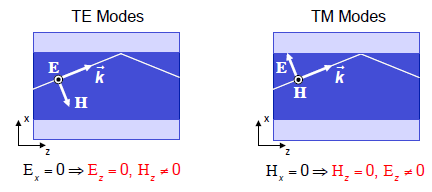
\includegraphics[scale=0.75]{ch1/image12}
	\captionof{figure}{ }
\end{center}


Nous allons considérer le mode TE\footnote{Je comprends pas trop pourquoi on fait ça ici.} tel que $E_x=0$. Les équations de Maxwell deviennent (voir Annexes)
\begin{equation}
{E_y} =  - \frac{{\beta {\rm{ }}\omega {\rm{ }}{\mu _0}}}{{{\gamma ^2} + {\beta ^2}}}{\rm{ }}{H_x}\qquad
{E_z} =  - \frac{{\gamma {\rm{ }}\omega {\rm{ }}{\mu _0}}}{{{\gamma ^2} + {\beta ^2}}}{\rm{ }}{H_x}\qquad
{H_y} =  - j\frac{\gamma }{{{\gamma ^2} + {\beta ^2}}}{\rm{ }}\frac{d}{{dx}}{H_x}\qquad
{H_z} =  - j\frac{\beta }{{{\gamma ^2} + {\beta ^2}}}{\rm{ }}\frac{d}{{dx}}{H_x}
\end{equation}
Une onde dans un guide infini est équivalent à une onde plane : pas de profil en $Y$ ou $Z$. On peut
alors définir $Z$ comme la direction dans laquelle se propage ce qui signifie que $\gamma=0$ car 
aucune phase n'est accumulée dans cette direction. Dès lors, $E_x=E_z=0$ (TE) et $H_y=0$)
\begin{equation}
{H_x} =  - \frac{{\beta {\rm{ }}}}{{\omega {\rm{ }}{\mu _0}}}{\rm{ }}{E_y},\qquad\qquad
{H_z} = \frac{{ - j}}{\beta }{\rm{ }}\frac{d}{{dx}}{H_x} = \frac{j}{{\omega {\rm{ }}{\mu _0}}}\frac{d}{{dx}}{E_y}
\end{equation}
où
\begin{equation}
\frac{{{d^2}{{\rm{E}}_y}}}{{d{x^2}}} + \left[ {\frac{{{\omega ^2}}}{{{c^2}}}{\kappa _j}(x) - {\beta ^2}} \right]{{\rm{E}}_y} = 0
\end{equation}
Faisons de même pour $H_x=0$. Nous avons $H_x=H_z=0$ (TM) et $E_y=0$ :
\begin{equation}
{E_x} = \frac{{\beta {\rm{ }}}}{{\omega {\rm{ }}{\varepsilon _0}{\rm{ }}\kappa }}{\rm{ }}{H_y}\qquad\qquad
{E_z} = \frac{{ - j}}{{\omega {\rm{ }}{\varepsilon _0}{\rm{ }}\kappa }}{\rm{ }}\frac{d}{{dx}}{H_y}
\end{equation}
où
\begin{equation}
\frac{{{d^2}{{\rm{H}}_y}}}{{d{x^2}}} + \left[ {\frac{{{\omega ^2}}}{{{c^2}}}{\kappa _j}(x) - {\beta ^2}} \right]{{\rm{H}}_y} = 0
\end{equation}

\cadre{\begin{center}
Un champ EM solution des équations de Maxwell dans un guide plan est une ainsi une \textbf{
combinaison linéaire} des modes TE et TM du guide d'onde.
\end{center}}\ \\


\subsubsection{Étape 2 : Résolution par milieu homogène}
Le guide d'onde est symétrique $\kappa(x)=\kappa(-x)$. L'intensité, proportionnelle au module carré 
$|E|^2$ est aussi symétrique. Les modes doivent alors être pairs ou impairs.\\

Intéressons-nous aux modes TE avec $\gamma=0$
\begin{equation}
\frac{{{d^2}{{\rm{E}}_y}}}{{d{x^2}}} + \left[ {\frac{{{\omega ^2}}}{{{c^2}}}{\kappa _j}(x) - {\beta ^2}} \right]{{\rm{E}}_y} = 0
\end{equation}
et plus particulièrement au cas où $E_y$ est symétrique (fonction paire de $x$). Il faut trouver une
solution symétrique satisfaisant les CL Dans la gaine $(|x|>a)$, nous voulons une atténuation afin d'avoir un maximum d'énergie dans le cœur
\begin{equation}
{{\rm{E}}_y} = {{\rm{A}}_{{\rm{sym}}}}\cos (\sigma a).\exp \left[ { - \xi (x - a)} \right]
\end{equation}
Dans le coeur $(|x|\leq a)$ nous pouvons avoir un cos ou un cosh. La seule solution acceptable est 
$\cos$ car elle respecte la continuité de la dérivée première\footnote{$H_z$ doit être continue et
elle dépend de la dérivée de $E_y$ par rapport à $x$.}
\begin{equation}
{{\rm{E}}_y} = {{\rm{A}}_{{\rm{sym}}}}\cos (\sigma x)
\end{equation}
La seule solution possible est un cos dans le cœur et une exponentielle décroissante dans la gaine. 
La continuité de $E_y$ en $x=a$ est alors vérifiée. 
\begin{center}
	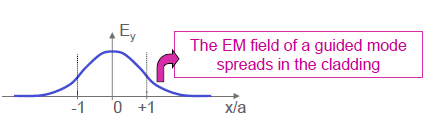
\includegraphics[scale=0.75]{ch1/image13}
	\captionof{figure}{ }
\end{center}

Dans les précédentes équations, nous avons posé
\begin{equation}
{\sigma ^2} = \frac{{{\omega ^2}}}{{{c^2}}}{\kappa _1} - {\beta ^2} = k_0^2n_1^2 - {\beta ^2}
\end{equation}
et
\begin{equation}
{\xi ^2} = {\beta ^2} - \frac{{{\omega ^2}}}{{{c^2}}}{\kappa _2} = {\beta ^2} - k_0^2n_2^2
\end{equation}
Quels sont les signes de $\sigma^2$ et $\xi^2$ ? 
\begin{itemize}
\item[$\bullet$] ${\sigma ^2} = k_0^2n_1^2 - {\beta ^2} > 0$ : $\sigma$ doit être réel pour 
satisfaire les CL
\item[$\bullet$] ${\xi ^2} = {\beta ^2} - k_0^2n_2^2 > 0$ : $\xi$ est réel. S'il est positif, on a
bien une décroissance exponentielle dans la gaine
\begin{equation}
\text{Mode quidé}\qquad\Leftrightarrow\qquad \beta > n_2k_0
\end{equation}
\item[$\bullet$] ${\xi ^2} = {\beta ^2} - k_0^2n_2^2 < 0$ : $\xi$ est imaginaire : oscillation 
dans la gaine
\begin{equation}
\text{Mode faible}\qquad\Leftrightarrow\qquad \beta^2> n_2^2k_0^2
\end{equation}
\end{itemize}\

Compte-tenu des conclusions ci-dessus, nousnaurons un mode quidé que si\\

\cadre{\textsc{Mode guidé si }\begin{equation}
n_nk_0>\beta > n_2k_0\qquad\Leftrightarrow\qquad n_1>n_2
\end{equation}}\ \\

Il s'agit bien ici d'un résultat, et non quelque chose que nous avons imposé comme c'était le cas
dans l'optique géométrique.


\subsubsection{Étape 3 : Condition de continuité à l'interface cœur-gaine}
Comme l'indique le nom de la sous-sous-section, il faut garantir la continuité de $H_z$ en 
$x=\pm a$, impliquant la continuité de la dérivée de $E_y$ en ce point. On trouve alors une 
branche de cosinus comme solution dans le cœur ($|x|\leq a$)
\begin{equation}
{H_z} = \frac{j}{{\omega {\rm{ }}{\mu _0}}}\frac{d}{{dx}}{E_y}\qquad\Rightarrow\qquad
{{\rm{H}}_z} =  - \frac{{j\sigma }}{{\omega \;{\mu _0}}}{{\rm{A}}_{{\rm{sym}}}}\sin (\sigma x)
\end{equation}
Et dans la gaine ($|x|>a$, déjà particularisé au point $a$)
\begin{equation}
{{\rm{H}}_z} =  \pm \frac{{ - j\xi }}{{\omega \;{\mu _0}}}{{\rm{A}}_{{\rm{sym}}}}\cos (\sigma a).\exp \left[ { - \xi (x - a)} \right]
\end{equation}
On en tire
\begin{equation}
 \pm \frac{{j\sigma }}{{\omega \;{\mu _0}}}{{\rm{A}}_{{\rm{sym}}}}\sin (\sigma a) =  \pm \frac{{j\xi }}{{\omega \;{\mu _0}}}{{\rm{A}}_{{\rm{sym}}}}\cos (\sigma a)
\end{equation}
D'où
\begin{equation}
\tan (\sigma a) = \frac{{\xi .a}}{{\sigma .a}}
\end{equation}

\begin{wrapfigure}[14]{l}{7.5cm}
	\vspace{-9mm}
	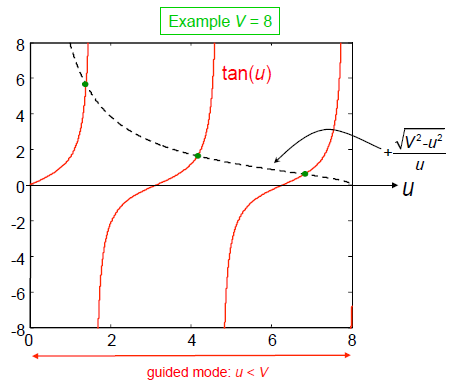
\includegraphics[scale=0.6]{ch1/image14}
	\captionof{figure}{3 solutions TE symétriques ($V=8$)}
	\end{wrapfigure}
Cette relation doit être vérifiée pour garantir la continuité. Toutes les solutions en termes de 
$\sigma$ vont être les solutions correspondant à un mode guidé. En posant les fonctions 
adimensionnelle $u \buildrel \Delta \over = \sigma .a = a.{(k_0^2n_1^2 - {\beta ^2})^{1/2}}$ et ${V^2} \buildrel \Delta \over = {a^2}({\xi ^2} + {\sigma ^2}) = {a^2}k_0^2(n_1^2 - n_2^2)$, on peut définir la \textbf{fréquence normalisée du guide d'onde}
\begin{equation}
V = a{k_0}\sqrt {n_1^2 - n_2^2} 
\end{equation}
où ${V^2} - {u^2} = {V^2} - {a^2}{\sigma ^2} = {a^2}{\xi ^2} > 0$ pour avoir un mode guidé ($\xi^2 > 0$ et $\xi > 0$). Physiquement, seule la valeur 
positive de $\xi$ convient sans quoi il y aurait une croissance infinie dans la gaine\\

\cadre{\begin{equation}
{\rm{tan(}}u{\rm{) =  + }}\frac{{\sqrt {{V^{\rm{2}}}{\rm{ -  }}{u^{\rm{2}}}} }}{u}
\end{equation}
Connaissant $\omega$ et l'index, il n'y a dès lors qu'un nombre \textbf{limité} de valeurs 
de $\sigma$ (et donc de $\beta$) satisfaisant à cette équation. Chaque $\beta$ \textbf{identifie}
un \textbf{mode guidé particulier}.}\ \\

Le même raisonnement peut être fait en partant d'un champ $E_y$ antisymétrique. On trouve alors\ \\

\cadre{\begin{equation}
{\rm{tan(u) =   -  }}\frac{{\rm{u}}}{{\sqrt {{{\rm{V}}^{\rm{2}}}{\rm{ -  }}{{\rm{u}}^{\rm{2}}}} }}
\end{equation}}\ \\

Ce qui est semblable à la précédente relation avec un signe négatif et une inversion 
numérateur/dénominateur\footnote{Voir slides 29-30 pour plus de détails.}. Pour $V=8$, il existe
également trois solutions TE, mais cette fois-ci antisymétriques. Comme la fonction rouge est 
tangente, il y aura toujours au moins un mode guidé. La fibre deviendra multimode dès la première
asymptote de cette fonction, à savoir en $u=\pi/2$.

\newpage
\begin{wrapfigure}[14]{l}{7.2cm}
	\vspace{-2mm}
	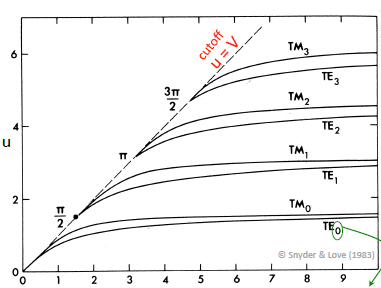
\includegraphics[scale=0.65]{ch1/image15}
	\captionof{figure}{ }
	\end{wrapfigure}
On peut faire le même calcul pour les modes $TM$ avec $\gamma=0 (E_x=E_z=H_y=0$). En évaluant la 
continuité, on retombe sur une équation aux valeurs propres pour les modes $TM$. Les conclusions
sont semblables : il y a toujours au moins un mode $TM$ et la valeur de la fréquence normalisée
à partir de la quelle on en voit d'autres est également $\pi/2$. \\

Le nombre de modes guidés augmente donc avec l'augmentation de la fréquence normalisée $V$. Dès 
lors, le guide est \textbf{monomode} si\\

\cadre{\begin{equation}
V < \dfrac{\pi}{2}
\end{equation}}\ \\

Les observateurs diront qu'il y a deux modes guidés en dessous de cette valeur (léger écart entre
$TE$ et $TM$). C'est vrai, mais on parle toujours de monomode : l'un ou l'autre sera excité en 
fonction de la polarisation. Ce léger écart signifie que le $\beta$ est différent pour les deux modes 
: le guide plan est \textit{biréfringeant}.

\subsubsection{Discussions}
\begin{enumerate}
\item \textit{Interprétation de $\beta$}.\\
Choisissons $z$ comme direction de propagation et $\gamma= 0$
\begin{equation}
{E_y} = {{\rm{E}}_y}\exp [j(\omega t - \beta z - \gamma y)] = {{\rm{E}}_y}\exp [j(\omega t - \beta z)]
\end{equation}
Le mode oscille à $\omega$ et accumule une phase dans la direction $z$ donnée par $\beta$ ($m^{-1}$). 
Il s'agit de la \textbf{constante de propagation} du mode. La variation de $\beta$ par rapport à la 
fréquence $\omega$, $\beta(\omega)$ est la \textbf{relation de dispersion du mode}. \\

Cette constante de propagation est bornée
\begin{equation}
\frac{{2\pi }}{{{\lambda _0}}}{n_2} < \beta  = \frac{{2\pi }}{{{\lambda _0}}}{n_{eff}} < \frac{{2\pi }}{{{\lambda _0}}}{n_1}
\end{equation}
où apparait l'indice effectif du mode, qui se rapporte à une mode tout comme $\beta$ : c'est 
l'indice de réfraction "vu" par le mode. Si un mode est fort dans la gaine, son indice effectif sera
proche de $n_2$ et inversement. En terme de vitesse de phase, le mode se propage à une vitesse entre
celle dans le cœur et celle dans la gaine
\begin{equation}
\frac{c}{{{n_1}}} < \frac{\omega }{\beta } < \frac{c}{{{n_2}}}
\end{equation}
La constante de propagation, via $\beta/\omega$, est alors fortement reliée à l'extension modale sur
le cœur et la gaine.
\newpage
\item \textit{Puissance par unité de longueur d'un mode TE}\footnote{Le guide plan étant infini
dans une direction transverse, il faut bien parler \textit{par unité de longueur}.}.
Celle-ci est donnée par l'intégrale de la composante $z$ du vecteur de Poynting moyennée 
temporellement sur $x$, celui-ci définissant la forme du guide
\begin{equation}
{P_u} = \int\limits_{ - \infty }^{ + \infty } {\left\langle {{S_z}} \right\rangle dx} 
\end{equation}
On en tire $\left\langle {{S_z}} \right\rangle  = \frac{\beta }{{2\;\omega \;{\mu _0}}}\;\;{E_y}{^2}$
et ${P_u} = 2\int\limits_0^{ + \infty } {\frac{\beta }{{2\;\omega \;{\mu _0}}}\;\;{E_y}{^2}dx}$. 
Pour les modes TE symétriques, en décomposant entre le cœur (première intégrale) et la gaine (la
seconde)
\begin{equation}
{P_u} = \frac{\beta }{{\omega \;{\mu _0}}}\left[ {\int\limits_0^a {\;{{({{\rm{A}}_{{\rm{sym}}}}\cos (\sigma x))}^2}dx + \int\limits_a^{ + \infty } {\;{{({{\rm{A}}_{{\rm{sym}}}}\cos (\sigma a).\exp \left[ { - \xi (x - a)} \right])}^2}dx} } } \right]
\end{equation}
On en tire
\begin{equation}
{P_u} = \frac{\beta }{{2\;\omega \;{\mu _0}}}{\rm{A}}_{{\rm{sym}}}^2[a + \frac{1}{\xi }]
\end{equation}
où ${h_{{\rm{eff}}}} \buildrel \Delta \over = {\rm{2(}}a{\rm{ + }}\frac{{\rm{1}}}{\xi }{\rm{)}}$ est
l'\textbf{épaisseur effective}. Tout se passe comme si l'énergie se réparti sur cette hauteur. Le
$1/\xi$ traduit bien l'étalement du mode sur la gaine optique, celui-ci n'étant pas bloqué dans le
cœur.
\item \textit{Profil transverse}\\
Considérons le cas précédemment abordé d'un mode $TE$ symétrique où $V=8$. La parité de l'indice 
donne une information sur la parité du mode, mais l'indice donne surtout le nombre de passage
par un zéro au sein du guide. Plus l'ordre du mode augmente, plus la complexité (nombre de nœud) du
mode fait de même. 

\begin{center}
	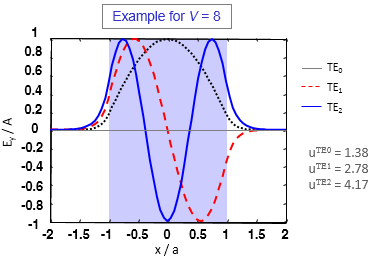
\includegraphics[scale=0.75]{ch1/image16}
	\captionof{figure}{ }
\end{center}

Notons que la partie évanescente du mode augmente avec l'ordre du mode lorsque $x$ diminue (l'indice
effectif se rapproche ainsi de $n_2$) : $\beta$ diminue avec l'ordre du mode.\\

Pour résumer, un grand $V$ implique un grand nombre de mode rimant avec une complexité d'onde guidée.
Il va y avoir superposition des modes guidés. Lorsqu'on excite plus d'un mode (TE/TM), l'intensité
devient dépendant de $z$ car $\beta^N$ diffère pour chaque ordre $N$. La simulation du \textit{slide 
35} met en évidence qu'un champ au début localisé se met à remplir tout le guide. Un champ évanescent
est en pratique toujours présent.\\

Intéressons-nous au profil transverse d'un mode \textit{près de la coupure}, par exemple en $V=1$. 
Plus on se rapproche de la coupure $(u=V$), plus $\xi$ est petit et plus l'extension du mode dans 
la gaine optique est importante (le profil modal étant proportionnel à $e^{-\xi}$, l'extention dans la
gaine augmente drastiquement). Ici, nous sommes
entre la coupure du mode 1 et 2. Par le calcul simple ${h_{{\rm{eff}}}}/(2a{\rm{)}} = {\rm{(1 + }}
\frac{{\rm{1}}}{{\xi .a}}{\rm{)  =  2}}{\rm{.47}}$, 
on voit que le mode est deux fois plus étendu dans le gaine que dans le cœur!
\begin{center}
	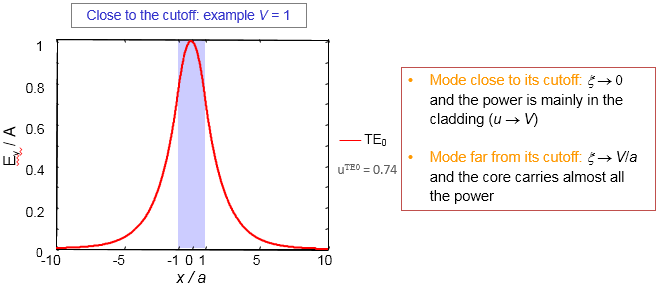
\includegraphics[scale=0.75]{ch1/image17}
	\captionof{figure}{ }
\end{center}
Nous sommes donc bien loin des considérations de l'optique géométrique. 

\item \textit{Interprétation du profil modal dans le cœur comme une superposition d'ondes planes}\\
Soit un mode TE symétrique d'ordre $N$
\begin{equation}
E_y^N = {{\rm{A}}_{{\rm{sym}}}}\cos ({u^N}.x/a).{e^{j(\omega t - {\beta ^N}z)}}
\end{equation}
Écrivons-le cosinus comme deux exponentielles 
\begin{equation}
E_y^N = \frac{1}{2}{{\rm{A}}_{{\rm{sym}}}}[{e^{j(\omega t - {\beta ^N}z + {u^N}.x/a)}} + {e^{j(\omega t - {\beta ^N}z - {u^N}.x/a)}}]
\end{equation}
On y voit deux ondes planes
\begin{equation}
{e^{j(\omega t - {\beta ^N}z - {u^N}.x/a)}} = {e^{j(\omega t - {k^N}.r)}}
\end{equation}
où $k_x^N = u^N/a, k_y^N=0$ et $k_z^N=\beta^N$. Calculons alors le module du nombre d'onde
\begin{equation}
\;k\;{^2} = {({u^N}/a)^2} + {({\beta ^N})^2} = {k_0}^2{n_1}^2 = {k_1}^2
\end{equation}
Celui-ci vaut $k_1^2$, soit exactement le nombre d'onde dans un milieu d'indice $n_1$ : il s'agit
d'une onde plane qui se propage.  La constante de propagation $\beta$ n'est que la projection de 
$\vec k_1$ sur la direction de propagation. 

\begin{center}
	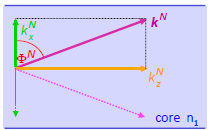
\includegraphics[scale=0.75]{ch1/image18}
	\captionof{figure}{ }
\end{center}

Le profil est le résultat des interférences entre
deux ondes planes de vecteur d'onde $(\pm k_x^N,0,\beta^N)$. On peut associer un "rayon" à une
onde plane (direction orthogonale au front d'onde, soit la direction de $k^N$) et retrouver la 
conclusion de l'optique géométrique 
\begin{equation}
\cos ({\Phi ^N}) = \frac{{{u^N}}}{{{k_1}.a}} < \frac{V}{{{k_1}.a}} = \frac{{a.{k_0}}}{{a.{k_0}.{n_1}}}\sqrt {{n_1}^2 - {n_2}^2}  = \sqrt {1 - {n_2}^2/{n_1}^2}  = \cos ({\Phi _c})\Rightarrow
\phi^N > \phi_c
\end{equation}

\item \textit{Ordre de grandeur}. Cf. \textit{slide 38}
\item \textit{Guide plan non symétrique}\\
Considérons $n_3$ comme étant de l'air : peu d'onde évanescante de ce côté, mais beaucoup de l'autre :
le mode est poussé du côté du saut d'indice le plus faible.
\begin{center}
	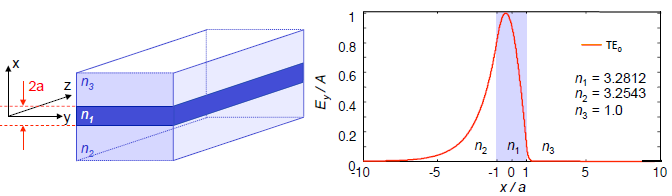
\includegraphics[scale=0.75]{ch1/image19}
	\captionof{figure}{ }
\end{center}
 Les solutions trouvées sont cependant
du même type.
\item \textit{Saut d'indice homogène dans un guide rectangulaire}. Pas de calcul analytique possible,
cf. \textit{slide 40}.
\end{enumerate}

\subsection{Guides à saut d'index cylindriques}
	\begin{wrapfigure}[9]{l}{6cm}
	\vspace{-5mm}
	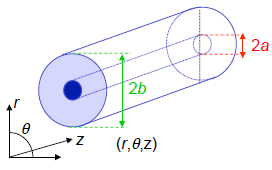
\includegraphics[scale=0.75]{ch1/image20}
	\captionof{figure}{ }
	\end{wrapfigure}
L'idée est la même, seule la géométrie va un petit peu compliquer les calculs ! La différence 
principale est que la structure a maintenant deux dimensions transverses : la propagation sera
caractérisée par deux paramètres. Faisons comme 
hypothèses
\begin{itemize}
\item[$\bullet$] Milieu diélectrique, non-magnétique, linéaire, isotropique et sans pertes
\item[$\bullet$] Milieu homogène (guide à saut d'indice, pas à gradient)
\item[$\bullet$] Gaine d'extension infinie ($2b\gg 2a$)
\end{itemize}
Encore une fois, il n'y a \textbf{pas} d'hypothèse sur la taille du cœur. \\

Nous avons dans le cœur ($r\leq a$)
\begin{equation}
\Delta {\bf{\tilde E}} + \kappa \left( \omega  \right)\frac{{{\omega ^2}}}{{{c^2}}}{\bf{\tilde E}} = 0,\qquad\qquad
\kappa \left( \omega  \right) = {n_1}^2\left( \omega  \right)
\end{equation}
Et dans la gaine ($r\geq a$)
\begin{equation}
\Delta \tilde H + \kappa \left( \omega  \right)\frac{{{\omega ^2}}}{{{c^2}}}\tilde H = 0,\qquad\qquad
\kappa \left( \omega  \right) = {n^2}_2\left( \omega  \right)
\end{equation}
Nous allons procéder à une résolution en considérant $E_z\neq 0$ et/ou $H_z\neq 0$ (voir 
\textit{Annexe 1}).

\subsubsection{Étape 1 : Propriété de symétrie, résolution par la méthode de séparation des variables}
La solution est une onde se propageant dans la direction $z$ où $\beta$ - la constante de 
propagation - joue le même rôle que précédemment.
\begin{equation}
\begin{array}{cc}
{E_z} = {\tilde E_z}(x,y)\exp (j[\omega t - \beta z]) & {H_z} = {\tilde H_z}(x,y)\exp (j[\omega t - \beta z])\\
\Downarrow & \Downarrow\\
\frac{{{\partial ^2}{{\tilde E}_z}}}{{\partial {x^2}}} + \frac{{{\partial ^2}{{\tilde E}_z}}}{{\partial {y^2}}} + [\kappa (\omega )\frac{{{\omega ^2}}}{{{c^2}}} - {\beta ^2}]{\tilde E_z} = 0
 & \frac{{{\partial ^2}{{\tilde H}_z}}}{{\partial {x^2}}} + \frac{{{\partial ^2}{{\tilde H}_z}}}{{\partial {y^2}}} + [\kappa (\omega )\frac{{{\omega ^2}}}{{{c^2}}} - {\beta ^2}]{\tilde H_z} = 0
\end{array}
\end{equation}
Vu la symétrie du problèmes, nous allons le traiter en symétrie cylindrique
\begin{equation}
x = r\cos (\theta ),\quad
y = r\sin (\theta ),\quad
r = \sqrt {{x^2} + {y^2}},\quad
\theta  = \arctan (\frac{y}{x})
\end{equation}
Dès lors, on trouve  $\frac{\partial }{{\partial x}} = \frac{x}{r}\frac{\partial }{{\partial r}} - \frac{y}{{{r^2}}}\frac{\partial }{{\partial \theta }}$ et $\frac{\partial }{{\partial y}} = \frac{y}{r}\frac{\partial }{{\partial r}} + \frac{x}{{{r^2}}}\frac{\partial }{{\partial \theta }}$. Nos 
champs s'écrivent
\begin{equation}
{\tilde E_r} = {\tilde E_x}\cos (\theta ) + {\tilde E_y}\sin (\theta ),\qquad\qquad
{\tilde E_\theta } =  - {\tilde E_x}sin(\theta ) + {\tilde E_y}\cos (\theta )
\end{equation}
En utilisant les nouvelles composantes de $\vec{E}$ et le Laplacien en coordonnées cylindriques, on 
trouve
\begin{equation}
\frac{{{\partial ^2}{{\tilde E}_z}}}{{\partial {r^2}}} + \frac{1}{r}\frac{{\partial {{\tilde E}_z}}}{{\partial r}} + \frac{1}{{{r^2}}}\frac{{{\partial ^2}{{\tilde E}_z}}}{{\partial {\theta ^2}}} + [\kappa (\omega )\frac{{{\omega ^2}}}{{{c^2}}} - {\beta ^2}]{\tilde E_z} = 0
\end{equation}
Et de même pour $H_z$. Actuellement, $\beta$ n'est pas connue. Nous allons chercher les solutions
physiquement acceptables et chercher à ce qu'elles satisfont les CL. Ceci fixera les valeurs de 
$\beta$ acceptable : elles formeront un ensemble discret, une valeur par mode.\\

Le problème à résoudre est donc
\begin{equation}
\left\{\begin{array}{l}
\DS \frac{{{\partial ^2}{{\tilde E}_z}}}{{\partial {r^2}}} + \frac{1}{r}\frac{{\partial {{\tilde E}_z}}}{{\partial r}} + \frac{1}{{{r^2}}}\frac{{{\partial ^2}{{\tilde E}_z}}}{{\partial {\theta ^2}}} + [\kappa (\omega )\frac{{{\omega ^2}}}{{{c^2}}} - {\beta ^2}]{\tilde E_z} = 0\vspace{2mm}\\
\DS\frac{{{\partial ^2}{{\tilde H}_z}}}{{\partial {r^2}}} + \frac{1}{r}\frac{{\partial {{\tilde H}_z}}}{{\partial r}} + \frac{1}{{{r^2}}}\frac{{{\partial ^2}{{\tilde H}_z}}}{{\partial {\theta ^2}}} + [\kappa (\omega )\frac{{{\omega ^2}}}{{{c^2}}} - {\beta ^2}]{\tilde H_z} = 0\DS\vspace{2mm}\\
\DS{\tilde E_r} =  - \frac{j}{{\kappa {\omega ^2}/{c^2} - {\beta ^2}}}\left( {\beta \frac{{\partial {{\tilde E}_z}}}{{\partial r}} + {\mu _0}\omega \frac{1}{r}\frac{{\partial {{\tilde H}_z}}}{{\partial \theta }}} \right)\DS\vspace{2mm}\\
\DS{\tilde E_\theta } =  - \frac{j}{{\kappa {\omega ^2}/{c^2} - {\beta ^2}}}\left( {\beta \frac{1}{r}\frac{{\partial {{\tilde E}_z}}}{{\partial \theta }} - {\mu _0}\omega \frac{{\partial {{\tilde H}_z}}}{{\partial r}}} \right)\DS\vspace{2mm}\\
\DS{\tilde H_\theta } =  - \frac{j}{{\kappa {\omega ^2}/{c^2} - {\beta ^2}}}\left( {\beta \frac{1}{r}\frac{{\partial {{\tilde H}_z}}}{{\partial \theta }} + \omega \;\varepsilon (\omega )\frac{{\partial {{\tilde E}_z}}}{{\partial r}}} \right)\DS\vspace{2mm}\\
\DS{\tilde H_r} =  - \frac{j}{{\kappa {\omega ^2}/{c^2} - {\beta ^2}}}\left( {\beta \frac{{\partial {{\tilde H}_z}}}{{\partial r}} - \omega \;\varepsilon (\omega )\frac{1}{r}\frac{{\partial {{\tilde E}_z}}}{{\partial \theta }}} \right)\DS
\end{array}\right.
\end{equation}
Auquel il faut joindre $\kappa(\omega)$ du cœur et de la gaine ainsi que les conditions de continuité
en $r=a$ de aux limites périodiques de $2\pi$ en $\theta$. On peut déjà souligner que $E_r$ dépend
de la dérivée de $E_z$ par rapport à $r$ et de $H_z$ par rapport à $\theta$ : les dérivées sont 
"mélangées" (cela aura de l'importance pour les CL).\\

Nous allons séparer la dépendance des solutions en $r$ et $\theta$ : ${\tilde E_z} = {R_z}(r)\;{\Theta
_z}(\theta )$, ce qui se justifie par la symétrie de rotation de la structure. On en tire
\begin{equation}
\frac{{{\partial ^2}{\Theta _z}}}{{\partial {\theta ^2}}} + {N^2}{\Theta _z} = 0,\qquad
\frac{{{\partial ^2}{R_z}}}{{\partial {r^2}}} + \frac{1}{r}\frac{{\partial {R_z}}}{{\partial r}} + [\kappa (\omega )\frac{{{\omega ^2}}}{{{c^2}}} - {\beta ^2} - \frac{{{N^2}}}{{{r^2}}}].\;{R_z} = 0
\end{equation}
où $N^2$ est positif pour avoir un terme oscillant, mais également la périodicité (celui-ci va 
définir la période du terme oscillant). Les fonction $\Theta_z$ et $R_z$ sont pour le moment 
inconnues.

\subsubsection{Étape 2 : Résolution du problème dans le cœur et la gaine optique}
La solution de l'équation azimutale (dépendance angulaire du champ) en $\Theta_z$ est une 
fonction harmonique à cause de la périodicité de $2\pi$ de la structure
\begin{equation}
\frac{{{\partial ^2}{\Theta _z}}}{{\partial {\theta ^2}}} + {N^2}{\Theta _z} = 0
\end{equation}
Dès lors, $N$ est forcément entier : c'est le nombre angulaire du mode
\begin{equation}
\;{\Theta _z}(\theta ) = \left\{ {\begin{array}{*{20}{c}}
{\cos (N\theta )}\\
{\sin (N\theta )}
\end{array}} \right.\qquad N= 0, \pm 1, \pm 2, \dots
\end{equation}
La seconde équation différentielle (partie radiale)
\begin{equation}
\frac{{{\partial ^2}{R_z}}}{{\partial {r^2}}} + \frac{1}{r}\frac{{\partial {R_z}}}{{\partial r}} + [\kappa (\omega )\frac{{{\omega ^2}}}{{{c^2}}} - {\beta ^2} - \frac{{{N^2}}}{{{r^2}}}].\;{R_z} = 0
\end{equation}
Peut s'écrire
\begin{itemize}
\item[$\bullet$] Si $\kappa\omega^2/c^2 - \beta^2 > 0$
\begin{equation}
{{\rm{x}}^2}\frac{{{d^2}{G_N}}}{{d{x^2}}} + x\frac{{d{G_N}}}{{dx}} + ({x^2} - {N^2}){G_N} = 0
\end{equation}
Si $N$ est entier, la dépendance radiale est une \textit{fonction de Bessel}
\item[$\bullet$] Si $\kappa\omega^2/c^2 - \beta^2 > 0$
\begin{equation}
{{\rm{x}}^2}\frac{{{d^2}{G_N}}}{{d{x^2}}} + x\frac{{d{G_N}}}{{dx}} - ({x^2} + {N^2}){G_N} = 0
\end{equation}
Si $N$ est entier, la dépendance radiale est une \textit{fonction de Bessel modifiée}
\end{itemize}
Notons que les deux conditions énoncées ici sont semblables à celle trouvée pour le guide plan.

\begin{center}
	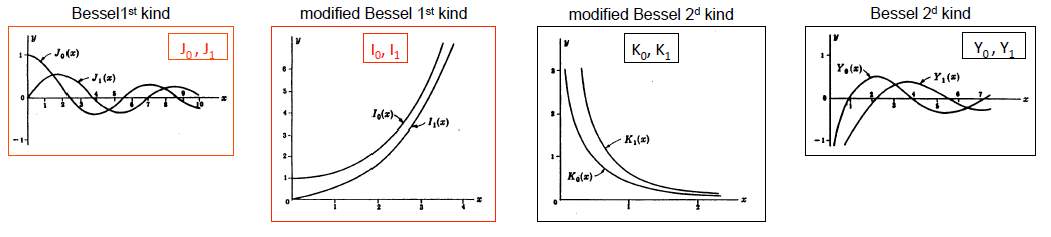
\includegraphics[scale=0.6]{ch1/image21}
	\captionof{figure}{La deuxième espèce diverge en 0. Dans le cœur, $J_k$ est acceptable mais pas 
$I_k$ à cause de la divergence. $I_k$ est également acceptable. Dans la gaine, $J_k$ 
n'est pas acceptable car la décroissance de l'amplitude est trop faible, mais $K_k$ est 
bon. Lesquelles prendre ? Nous avions vu que les dérivées étaient "mélangées". Comme 
$I_k$ donnerait un point anguleux, cette solution n'est pas acceptable. Nous avons 
finalement $J_k$ dans le cœur et $K_k$ dans la gaine.}
\end{center}

Pour $N$ fixé, un mode guidé est défini par\\

\cadre{\begin{equation}
\left\{\begin{array}{lll}
{R_z}(r) &= A{\vec{J}_N}(\sigma \;r)&\qquad \text{coeur } (x<a)\\
{R_z}(r) &= C{\vec{K}_N}(\xi \;r)&\qquad \text{gaine } (x\geq a)
\end{array}\right.
\end{equation}
Il s'agit de la \textbf{seule} solution possible (champ évanescent dans la gaine, pas de singularité,
champs continus en $x=a$).}\ \\

Pour avoir une solution dans le cœur, il faut que $\sigma^2>0 \Rightarrow n_1k_0>\beta$. Pour que
$K_n$ soit solution dans la gaine optique, il faut que $\xi^2>0 \Rightarrow \beta > n_2k_0$. Le 
mode ne sera guidé que si \\

\cadre{\begin{equation}
\frac{{2\pi }}{\lambda }{n_2} < \beta  < \frac{{2\pi }}{\lambda }{n_1}
\end{equation}
Soit encore $n_2<n_1$.}\ \\

Comme pour les guides d'ondes plan, la vitesse de phase $\omega/\beta$ dépend de 
l'extension sur le cœur \textbf{et} la gaine. Les solutions sont données aux \textit{slides 47} et \textit{48}.

\subsubsection{Classification des modes du nombre azimutal $N$}
\begin{enumerate}
\item Si $N=0$, il n'y a pas de dépendance angulaire. La situation est celle d'un guide plan et on retrouve les modes TE et TM formés par les rayons méridionaux.
\item Si $N\neq 0$, on ne retrouve pas de modes TE ou TM à causes des rayons obliques mais des \textbf{modes hybrides} $EH_{Nq}$ et $HE_{Nq}$. En fixant $N$, on trouvera alors $q$ solutions : se complique à cause des deux indices.
\end{enumerate}

\subsubsection{Étape 3 : Condition de continuité à l'interface cœur-gaine}
Il faut donc trouver pour un nombre azimutal $N$ donné, les $q$ solutions (nombre radial) possibles (s'il y en a). Le système est donné au \textit{slide 50}, mais "seulement" quatre équations sont indépendantes. Le système possède une solution non triviale ssi le déterminant du système est nul. A l'aide d'une insomnie, de l'hypothèse du \textbf{guidage faible} et de l'annexe 3, on trouve\\

\cadre{
\begin{equation}
\dfrac{\vec{J}_{m-1}(u)}{\vec{J}_{m}(u)}=-w\dfrac{\vec{K}_{m-1}(w)}{\vec{K}_{m}(w)}
\end{equation}
où
$$m=\left\{\begin{array}{lll}
1&\qquad\text{pour les modes $TE_{0q}$ et $TM_{0q}$}&\quad (N=0)\\
N+1&\qquad\text{pour les modes $EH_{Nq}$}&\quad (N\geq1)\\
N-1&\qquad\text{pour les modes $HE_{Nq}$}&\quad (N\geq1)
\end{array}\right.$$
}\ \\

Certains modes vont être caractérisés par le même $u$, et donc le même $\beta$ : ils sont dit
\textit{dégénérés} comme ils vont se propager avec la même constante de propagation. On va alors
les regrouper en remplaçant $N$ par $m$. Par exemple
\begin{description}
\item[m=0] correspond aux modes $TE_{0q}$ et $TM_{0q}$
\item[m=0] correspond au cas $N=1$ : seule possibilité est le mode $HE_{1q}$
\item[m=1] correspond aux modes $TE$ et $TM$ \textbf{mais aussi} au cas $N=2$ : $HE_{2q}$ à 
la même constante de propagation que $TE_{0q}$ et $TM_{0q}$.
\end{description}

On va alors écrire les combinaisons linéaires des modes dégénérés pour écrire les modes dits \textbf{
linearly polarized}, soit $LP_{mq}$. Dès lors, \textbf{pour chaque $m$ pour un $V$ fixé}, les $q$ 
solutions $u_{mq}$ de l'équation ci-dessus (et du $\beta_{mq}$ correspondant) donnent les $q$ 
modes $LP_{mq}$ guidés.\\

Considérons $V=2$ et $m=0,1$. Dans ce cas, la fibre est monomode mais elle deviendra multimode dès
le passage de l'asymptote pour $V=2.405$, soit le premier zéro de la fonction de Bessel : le mode
$LP_{11}$ sera alors guidé. Rappelons que $V^2=u^2+w^2$ : la condition de coupure $u=V$ implique que
$w=0$.

\begin{center}
	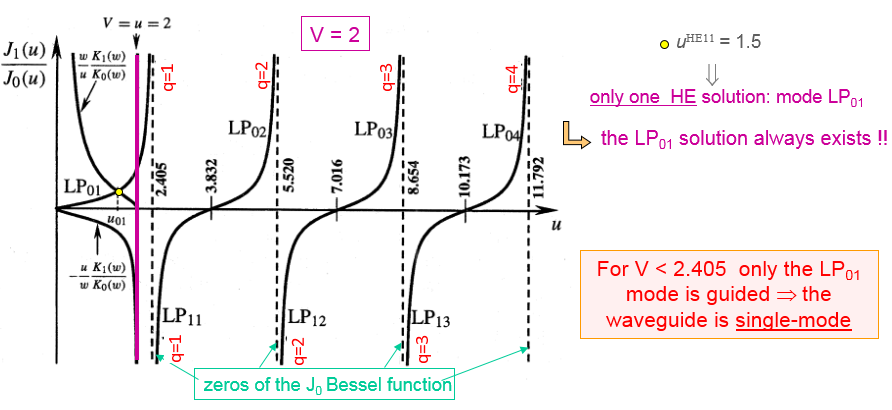
\includegraphics[scale=0.64]{ch1/image22}
	\captionof{figure}{ }
\end{center}

Considérons un second exemple où $V=8$
\begin{center}
	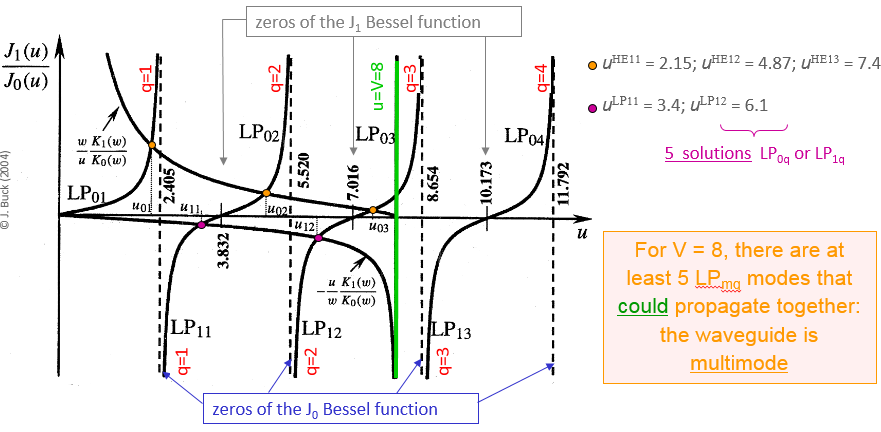
\includegraphics[scale=0.64]{ch1/image23}
	\captionof{figure}{ }
\end{center}
Dans ce cas, cinq modes $LP_{mq}$ peuvent être guidés en même temps : le guide d'onde est
multimode. Le tableau suivant résume la situation en nous informant de ce qui existe en fonction
de la valeur de $V$
\begin{center}
	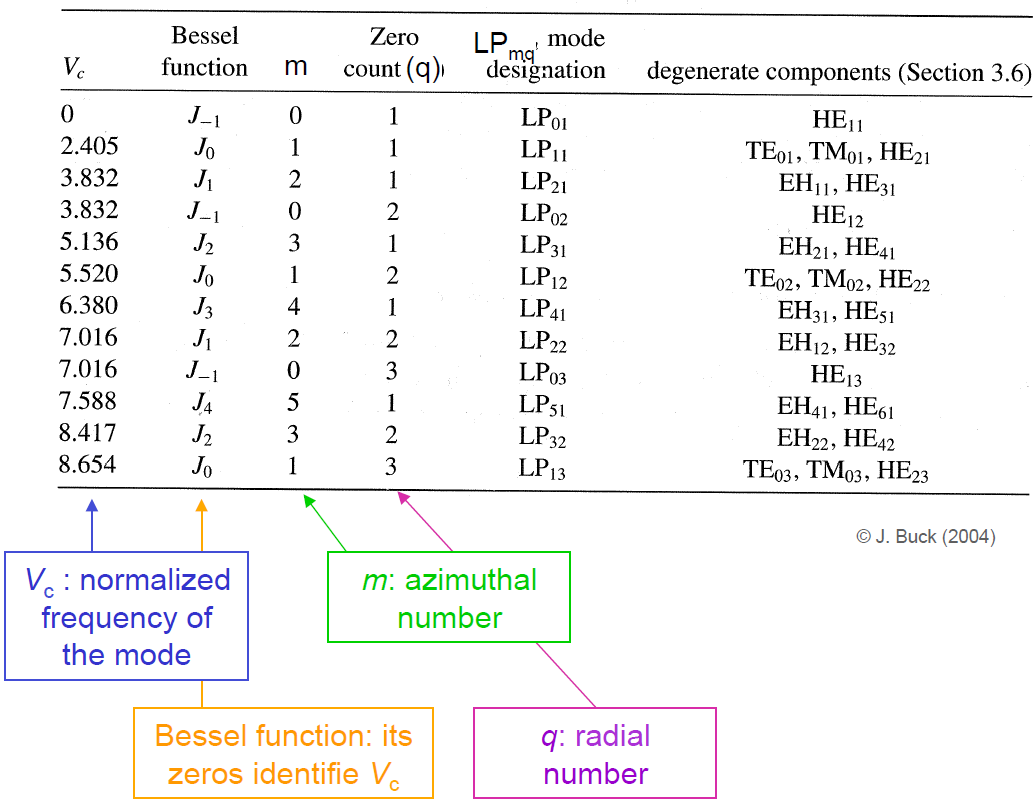
\includegraphics[scale=0.45]{ch1/tab1}
	\captionof{table}{ }
\end{center}



\subsubsection{Propriétés des modes $LP_{mq}$}
\begin{enumerate}
\item \textit{Distribution de l'intensité transverse $I(x,y)$}.\\
Dans le cas d'une fibre monomode, le seul mode guidé sera le $LP_{01} = HE_{11}$. D'autres exemples
sont donnés aux \textit{slides 55} et \textit{56}.
\begin{center}
	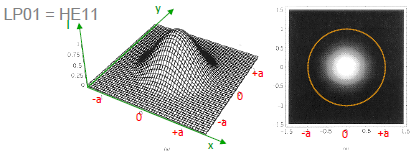
\includegraphics[scale=0.65]{ch1/image24}
	\captionof{figure}{ }
\end{center}
Soit le champ électrique du monde fondamental $LP_{01} = HE_{11}$ polarisé selon la direction 
$x$ ($E_y=0$). Son amplitude $|E_x|\propto J_0$ (cœur) et $|E_x|\propto K_0$ (gaine) est bien
approximée par une \textbf{distribution gaussienne} de paramètre $w_0$
\begin{equation}
{E_x}(r,z) = \exp [ - \frac{{{r^2}}}{{{w_0}^2}}].\exp [ - j\beta z]\quad\Rightarrow\quad
\frac{{{P_{core}}}}{{{P_{total}}}} = 1 - \exp [ - \frac{{2{a^2}}}{{{w_0}^2}}]
\end{equation}
Ceci est vrai pour autant que l'on ne se situe pas trop près de la coupure du mode ($V=0$ pour
le fondamental)
\newpage
\begin{center}
	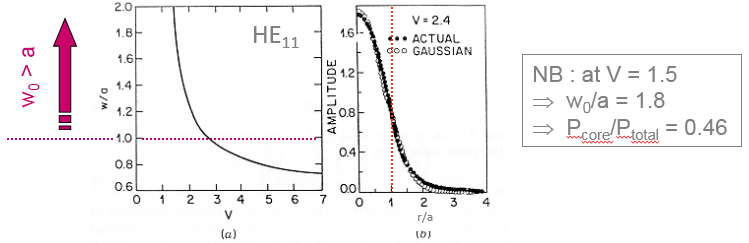
\includegraphics[scale=0.55]{ch1/image25}
	\captionof{figure}{Bon accord entre le fit gaussien et le mode analytique}
\end{center}
On va alors définir le \textbf{Mode Field Diameter (MFD)} $=2w_0$ comme un paramètre du mode
fondamental.\\

Malgré la symétrie cylindrique, il est plus simple de représenter les polarisations linéaires
dans un repère cartésien
\begin{equation}
{E_x} = {E_r}\cos (\theta ) - {E_\theta }\sin (\theta ) = 0,\quad
{E_y} = {E_r}\sin (\theta ) + {E_\theta }\cos (\theta ) = A( - j\beta \frac{a}{u}){\vec{J}_0}(\frac{{u.r}}{a}).\exp (j[\omega t - \beta z])
\end{equation}
Le mode $LP_{01}$ est ainsi polarisé linéairement (a)
\begin{center}
	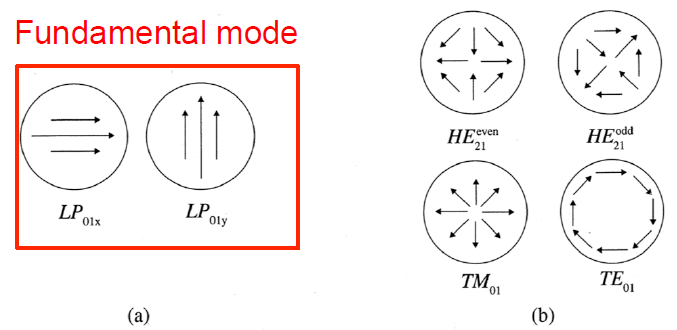
\includegraphics[scale=0.4]{ch1/image26}
	\captionof{figure}{ }
\end{center}
En (b), il faudra considérer la combinaison linéaire entre ces quatre modes-là pour former le 
mode $LP_{11}$. Il existe différentes combili et donc différents résultats possibles qui sont
illustrés au \textit{slide 58}.\\

\item \textit{Confinement de l'intensité}.\\
Le graphique ci-dessous montre la répartition de la puissance entre le cœur et la gaine optique
à l'aide de $\psi$
\begin{equation}
\psi  = \frac{{{P_{cladding}}}}{{{P_{cladding}} + {P_{core}}}}
 = \left( {\frac{{{u^2}}}{{{V^2}}}} \right)\left( {1 - \frac{{\vec{{\rm K}}_m^2(w)}}{{{\vec{{
 \rm K}}_{m - 1}}(w).{\vec{{\rm K}}_{m + 1}}(w)}}} \right)
\end{equation}
pù $0<\psi<1$.
\newpage
\begin{center}
	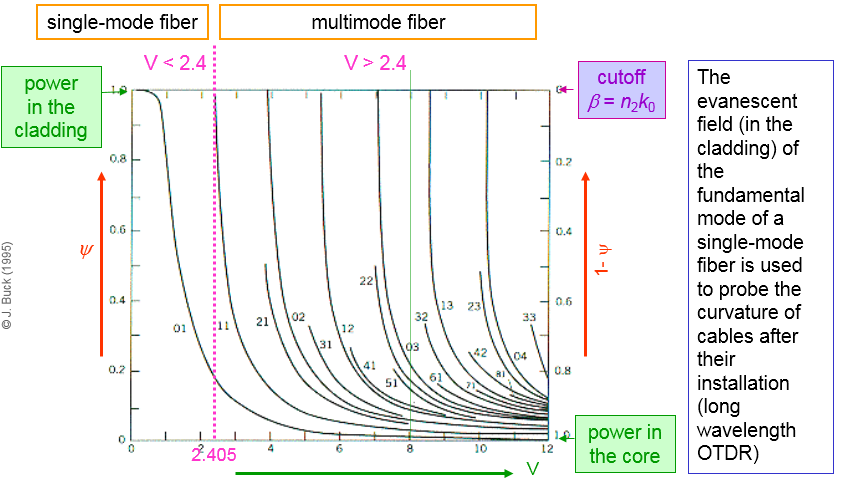
\includegraphics[scale=0.54]{ch1/image27}
	\captionof{figure}{ }
\end{center}
Pour monitorer les pertes, on envoie une onde dans la fibre et on mesure la partie réfléchie
(qui revient à l'entrée) en fonction du temps : permet la détermination des pertes locales (par
exemple, une grosse courbure). Une chute de puissance peut être causée par le passage de la fibre
dans un coin, celle-ci est alors trop tordue. Plus le mode s'étale dans la gaine, plus il est 
sensible aux courbures\footnote{Note en vrac : $V = \frac{2\pi}{\lambda}\sqrt{n_1^2-n_2^2}$, plus
la longueur d'onde est grande, plus $V$ est petite.}.\\

\item \textit{Courbes de dispersions}.\\
En introduisant la constante de propagation normalisée
\begin{equation}
b = 1 - \frac{{{u^2}}}{{{V^2}}} = \frac{{{\beta ^2} - {k_0}^2{n_2}^2}}{{{k_0}^2{n_1}^2 -
 {k_0}^2{n_2}^2}} = \frac{{{n_{eff}}^2 - {n_2}^2}}{{({n_1}^2 - {n_2}^2)}}
\end{equation}
où $0<b<1$. Si $b$ est proche de 0 c'est que l'on est proche de la coupure : mode totalement dans la
gaine, l'indice "vu" va être comme si tout le mode était dans la gaine. Si $b=1$, la conclusion est 
inverse. Notons que nous ne faisons ici que changer $V$ et pas $n_1$ et $n_2$.
\begin{center}
	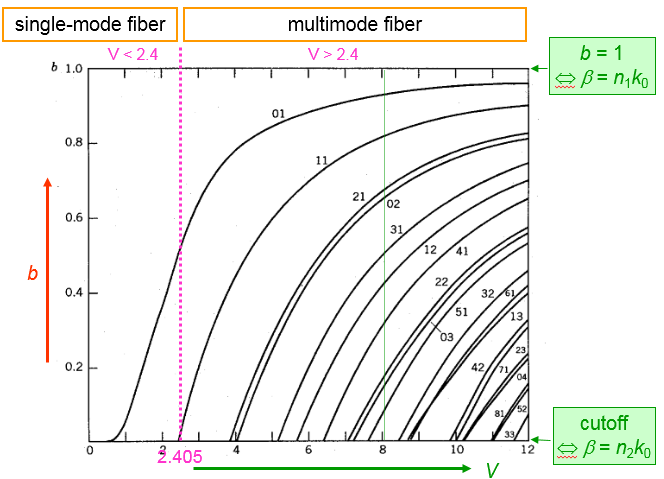
\includegraphics[scale=0.4]{ch1/image28}
	\captionof{figure}{ }
\end{center}\ \\

\item \textit{Mais aussi}\dots\\
Une fibre est monomode si seulement le monde fondamental est guidé
\begin{equation}
V = \frac{{2\pi }}{\lambda }a\sqrt {n_1^2 - n_2^2}  < 2.405
\end{equation}
où $\lambda > \lambda_{cutoff}, \sqrt{\dots} \approx 5\mu$m $\Delta n \approx 3\times 10^{-3}$. Un
paramètre important est le \textbf{Mode Field Diameter (MFD)} : lors de la soudure de fibres, il 
faut que les MFD soient proches sinon pleins de pertes vont être introduites. Plus le MFD est 
petit, plus l'intensité est localement importante. En pratique, on utilise un MFD un peu plus grand
que la valeur "idéale" pour éviter d'injecter trop de puissance et avoir trop d'effets non linéaires.
\end{enumerate}

\section{Fabrication des fibres optiques}
Voir \textit{slides 69} à \textit{75} ainsi que la vidéo sur l'UV.


\newpage
\section{Propriétés linéaires des fibres optiques}
\subsection{Atténuation du signal dans les fibres monomodes}
	\begin{wrapfigure}[5]{l}{10cm}
	\vspace{-5mm}
	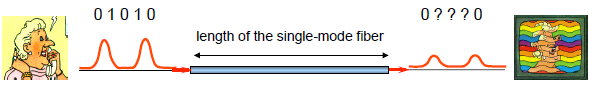
\includegraphics[scale=0.6]{ch1/image29}
	\captionof{figure}{ }
	\end{wrapfigure}
Quand un signal se propage dans une fibre, plusieurs éléments vont jouer en la défaveur de 
celui-ci. La fibre n'est pas parfaite et possède des \textbf{pertes}. Le problème est qu'un 
détecteur possède une sensibilité limitée : un puissance minimale doit l'atteindre, ce qui va
limiter la distance de propagation. \\

Les pertes par propagation sont caractérisée par la le \textbf{coefficient d'atténuation} 
$\alpha$, liée à la partie imaginaire de la susceptibilité $\chi(\omega)$ (alors que la partie
réelle donne plutôt l'indice de réfraction).\\

	\begin{wrapfigure}[8]{r}{8.5cm}
	\vspace{-12mm}
	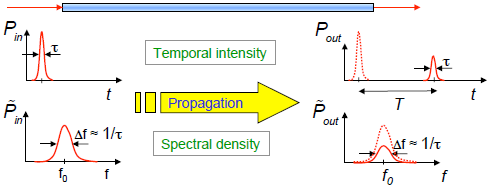
\includegraphics[scale=0.65]{ch1/image30}
	\captionof{figure}{ }
	\end{wrapfigure}
	
	Étudions la propagation d'un \textit{pulse} dans une fibre optique. Que ce soit dans le 
	domaine temporel ou spectral, on observe une diminution de l'amplitude de celui-ci, mais
	pas un élargissement. Cette diminution est exprimée via la loi de Beer-Lambert
	\begin{equation}
	\dfrac{dP(z)}{dz} = -\alpha_mP\qquad\Rightarrow\qquad P(L) = P(0)\exp(-\alpha_mL)
	\end{equation}
	où $\alpha_m$ est le coefficient d'atténuation ($[m^{-1}]$), $P(z=L)$ la puissance de 
	sortie et $P(z=0)$ la puissance d'entrée. On en tire\\
	
	\cadre{\begin{equation}
	\alpha[\text{dB/km}] \equiv -\dfrac{10}{1\text{ km}}\log_{10}\left(\dfrac{P(z=\text{ 1km})}{
	P(z=0)}\right)
	\end{equation}}\ 
	
	Si l'on souhaite l'atténuation en amplitude, on utilisera la relation
	\begin{equation}
	\alpha[\text{dB/km}]\times\text{1 km} = 10\log_{10}(e)\times\alpha_m\times1\text{km} = 
	4.343\times\alpha_m\times\text{1 km}
	\end{equation}

	Il existe trois sources d'atténuation dans une fibre (cf. figure ci-dessous)
	\begin{enumerate}
	\item  \textbf{Absorption matérielle}\\
	Lorsque la lumière se propage dans la matière, il va y avoir de l'absorption causant
	une excitation des modes de vibration et rotation. On retrouve ces absorptions dans 
	l'infrarouge, en mauve sur le graphique.\\
	
	Lors de la fabrication des fibres, il peut se glisser autre chose que de la silice : 
	elle peut être polluée par de ions $OH^-$ qui viennent de l'eau (air, vapeur, \dots). 
	Cela va introduire des pics d'absorption.\\
	
	\item \textbf{Diffusion de Rayleigh}\\
	Inévitable car en présence d'un matériau amorphe. Les fluctuation de densité vont créer
	de la diffusion. On remarque que Rayleigh (rouge pointillé) est non-négligeable par 
	rapport à l'absorption de la fibre en elle-même\footnote{Pour info, $\alpha_R \approx 0.16$
	dB/km à $\lambda = 1.5\mu m$.}.\\
	
	\item \textbf{Radiations dues aux imperfection dans le guide}.\\
	La fibre peut présenter des courbures. Si celles-ci sont trop importantes, l'angle d'incidence
	est trop petit et on va radier de l'énergie : la réflexion est partielle. Plus le rayon de 
	courbure est petit, plus on est couplé à de l'énergie radiée. Cela dépend fortement de la fibre
	et la longueur d'onde.	\\
	
	On retrouve aussi les pertes dues à une pression sur la fibre, créant des micro-courbures
	qui ont tendance à faire radier l'énergie. Les connecteurs et le \textit{splicing} de fibre
	introduisent également des pertes.
	\end{enumerate}

	\begin{wrapfigure}[11]{l}{10cm}
	\vspace{-5mm}
	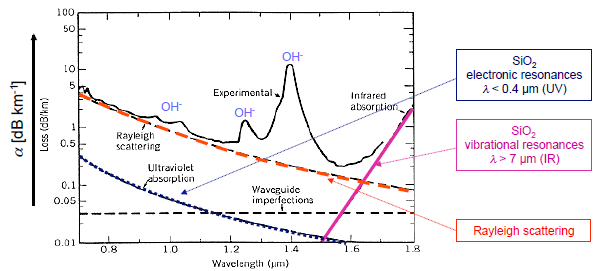
\includegraphics[scale=0.6]{ch1/image31}
	\captionof{figure}{ }
	\end{wrapfigure}
	De façon générale, on voit un minimum d'atténuation $\lambda \approx 1550$ nm et c'est la 
	raison de l'utilisation de cette longueur d'onde en télécommunication. Historiquement on 
	travaillait à 1300 nm (entre les deux pics d'$OH^-$) car la dispersion chromatique était
	plus faible ce qui permettait la propagation sur une plus longue distance.\\
	
	L'atténuation totale est donnée par
	\begin{equation}
	\text{Atténuation (dB)} = \sum_i\alpha_iL_i+\alpha_sx+\alpha_cy+\alpha_b
	\end{equation}
	où $\alpha_b$ est négligeable (pertes par pression).
	
	
	\subsection{Dispersion chromatique}
	Dans le cas d'une fibre mono-mode ($V = k_0a\sqrt{n_1^2-n_2^2} < 2.405$), le dispersion 
	inter-modale n'est pas problématique (logique, seul $LP_{01}$ se propage). Cependant, un
	pulse lors de sa propagation peut subir le \textbf{dispersion de vitesse de groupe}\footnote{
	Ou "dispersion intra-modale", "dispersion de fibre", "dispersion chromatique".}. \\
	
	Celle-ci vient 
	\begin{enumerate}
	\item Le spectre à largeur finie du signal (modulation et source)
	\item L'indice de réfraction $n$ de la silice varie en fonction de la fréquence (c'est d'ailleurs
	ce qui permet à un prise en silice de décomposer la lumière). C'est la \textbf{dispersion 
	matérielle}.
	\item La constante de propagation $\beta$ dépend de la longueur d'onde (changer $\lambda$ change
	$V$ et changer $V$ augmente l'étalement spectral : $\beta$ change). On parle ici de 
	\textbf{dispersion du guide}.
	\end{enumerate}
	
	\newpage
	\begin{wrapfigure}[11]{l}{8cm}
	%\vspace{-5mm}
	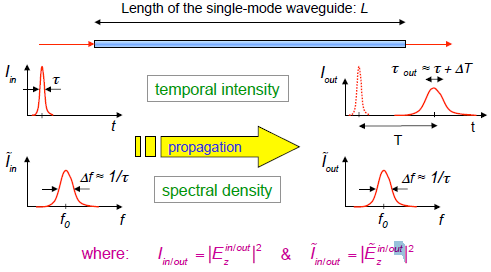
\includegraphics[scale=0.6]{ch1/image32}
	\captionof{figure}{ }
	\end{wrapfigure}	
	Dans le domaine temporel, la dispersion chromatique cause une diminution de l'amplitude du
	pulse ainsi qu'un étalement du spectre. Par contre, pas de changement notable dans l'intensité
	spectrale : on verra plus tard que la phase spectrale, elle, se modifie. Rappelons l'expression
	de la vitesse de groupe
	\begin{equation}
	v_g = \left(\dfrac{d\beta}{d\omega}\right)^{-1} = \dfrac{c}{n_g} \quad\Rightarrow\quad
	T = \dfrac{L}{v_g}
	\end{equation}
	où $n_g$ est l'indice de groupe et $T$ le temps de vol du pulse. C'est parce que la vitesse
	de groupe n'est \textbf{pas la même pour toutes les fréquences du spectre du pulse} que sa
	largeur augmente lorsqu'il se propage dans la fibre.\\
	
	Calculons l'étalement temporel $\Delta T$ du pulse (lié donc à la différence de vitesse de 
	propagation). Soit $\Delta \omega$, le spectre lié à l'information qui transite. La variation
	du temps de vol est donné par la variation de fréquence $dT/d\omega\Delta \omega$. On trouve
	alors un coefficient qui dépend de la dérivée seconde
	\begin{equation}
\Delta T = \frac{{dT}}{{d\omega }}\Delta \omega  = \frac{d}{{d\omega }}\left( {\frac{L}{{{v_g}}}} \right)\Delta \omega  = L\frac{{{d^2}\beta }}{{d{\omega ^2}}}\Delta \omega  = L{\beta _2}\Delta \omega 
	\end{equation}
	On peut écrire une équation semblable, mais avec $\Delta \lambda$, lié aux longueurs d'ondes de
	l'information qui transite
	\begin{equation}
\Delta T = \frac{d}{{d\lambda }}\left( {\frac{L}{{{v_g}}}} \right)\Delta \lambda  = LD\Delta \lambda  = LD\frac{{ - {\lambda ^2}}}{{2\pi c}}\Delta \omega 
	\end{equation}
	On en tire un lien entre $D$ et $\beta_2$ (\danger\ signe différent, important car les effets
	sont différents!)
	\begin{equation}
D =  - \frac{{2\pi c}}{{{\lambda ^2}}}{\beta _2}
	\end{equation}
	où $D$ est la paramètre \textit{GVD} et $D$ le paramètre de dispersion (ps. nm$^{-1}$.km$^{-1}$).
	Physiquement, le paramètre important est $\beta_2$ mais dans les calculs de type ingénieur où il
	faut avoir rapidement des ordres de grandeur on utilisera plutôt $D$. En résumé\\
	
	\cadre{\begin{equation}
{\beta _2} = \frac{{{d^2}\beta }}{{d{\omega ^2}}},\qquad\qquad\qquad
D = \frac{d}{{d\lambda }}(\frac{1}{{{v_g}}}) =  - \frac{{2\pi c}}{{{\lambda ^2}}}{\beta _2}
	\end{equation}}\ \\
	
	On peut estimer la limitation du produit $BL$ par la dispersion chromatique. Si l'écart temporel
	reste inférieur au temps d'un bit, l'information peut être retrouvée. En définissant le temps
	bit $T_B$ comme l'inverse du débit binaire, on trouve que
	\begin{equation}
BL < \frac{1}{{\left| D \right|\Delta \lambda }}
	\end{equation}
	où $\Delta \lambda$ est le contenu spectral, ici de la \textbf{source laser} et non de la 
	modulation! D'où l'importance de travailler avec un laser suffisamment cohérent. En résumé, 
	trois contribution
	\begin{enumerate}
	\item \textbf{Dispersion matérielle} : $n=n(\omega)\to D_M$
	\item \textbf{Dispersion de profil} : $\Delta=\Delta(\omega)$ (le saut d'indice peut varier
	en fonction de la longueur d'onde). En pratique, négligeable
	\item \textbf{Dispersion du guide} : $\beta=\beta(\omega)\to D_W$	
	\end{enumerate}

	\begin{equation}
	D = D_M + D_W
	\end{equation}
		\begin{wrapfigure}[13]{l}{11cm}
	%\vspace{-5mm}
	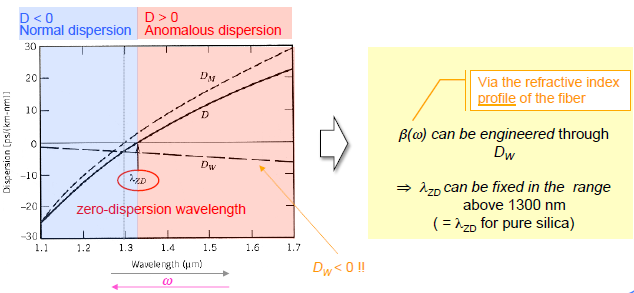
\includegraphics[scale=0.6]{ch1/image33}
	\captionof{figure}{ }
	\end{wrapfigure}	
	On peut voir ci-contre que la dispersion du guide est toujours négative. La dispersion totale 
	($D$) sera un peu "shiftée" vers le bas. Le zéro de dispersion ne va pas se situer au zéro de
	la silice mais un peu au dela. Comme on peut jouer sur $\beta(\omega)$ via $D_W$, on va pouvoir
	fixer $\lambda_{ZD}$.  On parlera alors de fibre DSF (Dispersion-Shifted Fiber) : on amène le
	zéro de dispersion à 1.5 micron afin d'avoir le minimum de pertes et de dispersion. Cependant,
	travailler à $\lambda_{ZD}$ n'est pas toujours bien (effets non-linéaires). On travaille alors
	un peu plus loin : fibres à dispersion décallée mais non nulle NZDSF (Non-Zero Dispersion-Shifted
	Fiber).\\
	
	Essayons d'établir l'équation de propagation d'un pulse. Nous allons faire l'approximation de
	l'enveloppe lentement variable (SVEA) signifiant que $\Delta \omega\ll \omega_0$ où 
	$\omega_0$ est la fréquence de la porteuse. On fera aussi les hypothèses
	\begin{enumerate}
	\item Le mode $LP_{01}$ est polarisé linéairement selon la direction $x$
	\item Guidage faible $\Delta n \ll 1 \Rightarrow |E_z|\ll |E_x|$ (champ quasi transverse)
	\item Le profil modal est identique pour toutes les composantes spectrales du signal
	\item Milieu sans pertes et linéaire
	\end{enumerate}

	Décrivons notre problème en fonction du champ $\vec{E}$. Pour une onde monochromatique
	\begin{equation}
	{E_x}(x,y,z,t) = F(\rho ).\Theta (\theta ).B(z,t)
	\end{equation}
	où $B(z,t) = \tilde b.\exp (j[{\omega _0}t - {\beta _0}z])$ avec la porteuse et $\beta_0$, la 
	constante de propagation à $\omega_0$. \\
	Pour les ondes polychromatiques comme les pulses, on notera
	\begin{equation}
	{E_x}(x,y,z,t) = F(\rho ).\Theta (\theta )\underbrace{\int {\tilde b(\omega ).\exp (j[\omega t - \beta (\omega )z])} .d\omega }_{B(z,t)}
	\end{equation}
	où $|\tilde b(\omega )|^2 \propto$ la densité spectrale. \\
	
	Effectuons l'approximation de l'\textbf{enveloppe lentement variable} (SVE) $A(z,t)$
	\begin{equation}
	B(z,t) = A(z,t).\exp \left( {j[{\omega _0}t - {\beta _0}z]} \right)
	\end{equation}
	où la largeur spectrale de $\tilde{A}$ est $\ll \omega_0$. Effectuons la transformée de Fourier
	par rapport à $\omega$
	\begin{equation}
\tilde B(z,\omega ) = \int\limits_{ - \infty }^{ + \infty } {B\exp ( - j\omega t)dt}  = \int\limits_{ - \infty }^{ + \infty } {A(z,t).\exp \left( {j[{\omega _0}t - {\beta _0}z]} \right)\exp ( - j\omega t)dt} 
 = \tilde A(z,\omega  - {\omega _0}).\exp \left( { - j{\beta _0}z} \right)
	\end{equation}
	Prenons la TF de cette expression par rapport à $\beta$
	\begin{equation}
\tilde B(\beta ,\omega ) = \int\limits_{ - \infty }^{ + \infty } {\tilde B(z,\omega )\exp ( + j\beta z)dz} 
 = \tilde A(\beta  - {\beta _0},\omega  - {\omega _0})
	\end{equation}
	Développons la constante de propagation $\beta(\omega)$ jusqu'à l'ordre 3 autour de la fréquence
	de la porteuse $\omega_0$
	\begin{equation}
\beta \left( \omega  \right) \approx {\beta _0} + {\beta _1}\left( {\omega  - {\omega _0}} \right) + \frac{1}{2}{\beta _2}{\left( {\omega  - {\omega _0}} \right)^2} + \frac{1}{6}{\beta _3}{\left( {\omega  - {\omega _0}} \right)^3} + ...
	\end{equation}
	où $\DS {\beta _m} = {\left. {\left( {\frac{{{d^m}}}{{d{\omega ^m}}}\beta } \right)} \right|_{\omega  = {\omega _0}}}$. Multiplions ce développement par la résultat de notre précédente TF
	\begin{equation}
	(\beta  - {\beta _0})\tilde A(\beta  - {\beta _0},\omega  - {\omega _0}) - \left[ {{\beta _1}(\omega  - {\omega _0}) + \frac{1}{2}{\beta _2}{{(\omega  - {\omega _0})}^2} + \frac{1}{6}{\beta _3}{{(\omega  - {\omega _0})}^3}} \right]\tilde A = 0
	\end{equation}
	Par changement de variable $\beta'=\beta-\beta_0$ et $\omega' = \omega-\omega_0$
	\begin{equation}
	\beta '\tilde A(\beta ',\omega ') - ({\beta _1}\omega ' + \frac{1}{2}{\beta _2}\omega {'^2} + \frac{1}{6}{\beta _3}\omega {'^3})\tilde A = 0
	\end{equation}
	En effectuant la transformée de Fourier inverse en $\beta'$
	\begin{equation}
	\frac{\partial }{{\partial z}}\tilde A(z,\omega ') =  - j({\beta _1}\omega ' + \frac{1}{2}{\beta _2}\omega {'^2} + \frac{1}{6}{\beta _3}\omega {'^3})\tilde A
	\end{equation}
	Au second ordre, la propagation dans un milieu linéaire dispersif cause seulement une 
	évolution quadratique de la phase du champ : la \textbf{phase spectrale} est \textbf{quadratique}.
	La densité spectrale $|\tilde{B}|^2$ reste elle bien constante (sans pertes, linéaire).\\
	
	Pour retrouver la propagation dans le domaine temporel, il faut effectuer la transformée de 
	Fourier inverse en $\omega'$. L'\textbf{évolution de l'enveloppe lentement variable $A$} est
	donnée par 
	\begin{equation}
	\frac{{\partial A(z,t)}}{{\partial z}} + {\beta _1}\frac{{\partial A}}{{\partial t}} - j\frac{{{\beta _2}}}{2}\frac{{{\partial ^2}A}}{{\partial {t^2}}} - \frac{{{\beta _3}}}{6}\frac{{{\partial ^3}A}}{{\partial {t^3}}} = 0
	\end{equation}
	En nous mettant dans le référentiel temporel du pulse ($t'=t-\beta_1z, z'=z$)\\
	
	\cadre{\begin{equation}
	\frac{{\partial A}}{{\partial z'}} - j\frac{{{\beta _2}}}{2}\frac{{{\partial ^2}A}}{{\partial t{'^2}}} - \frac{{{\beta _3}}}{6}\frac{{{\partial ^3}A}}{{\partial t{'^3}}} = 0
	\end{equation}
	où le second terme est la \textbf{G}roup \textbf{V}elocity \textbf{D}ispersion (GVD).}\ \\
	
	Les slides 93 et 94 donnent des exemples de dispersion. Essayons d'interpréter ces résultats. 
	A cause de la dispersion chromatique, l'expression de la vitesse de groupe devient
	\begin{equation}
	{v_g}(\omega ) = \frac{1}{{{{[d\beta } \mathord{\left/
 {\vphantom {{[d\beta } {d\omega }}} \right.
 \kern-\nulldelimiterspace} {d\omega }}{]_{{\omega _0}}} + {\beta _2}(\omega  - {\omega _0})}}
	\end{equation}
	On voit apparaître un $+\beta_2$ : les fréquences décalées vers le bleu (fréquences élevées) 
	vont se propager plus vite.
	\newpage
	
	\begin{wrapfigure}[18]{l}{10cm}
	%\vspace{-5mm}
	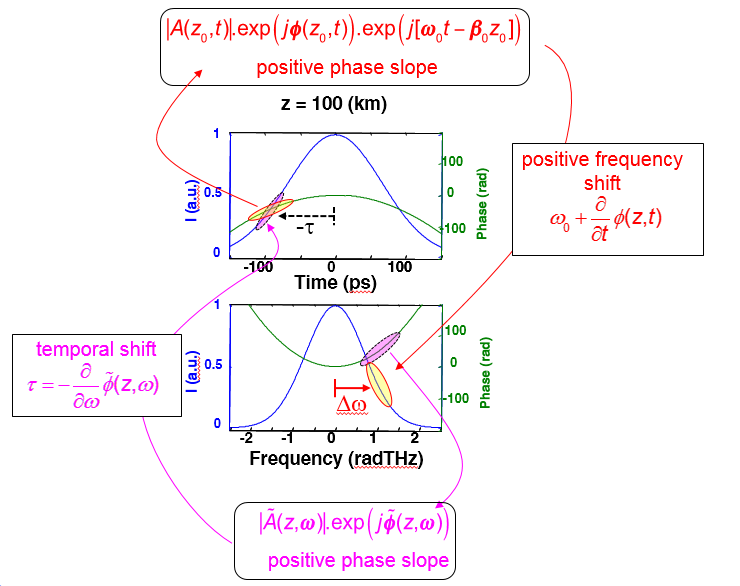
\includegraphics[scale=0.5]{ch1/image34}
	\captionof{figure}{ }
	\end{wrapfigure}
	Considérons la représentation spectrale. La pente de de la phase du groupe de fréquence mauve
	est positive : il en résulte un shift temporel donné par
	\begin{equation}
	\tau  =  - \frac{\partial }{{\partial \omega }}\tilde \phi (z,\omega )
	\end{equation}
	Ici la pente est positive, le délai introduit est donc négatif : ces fréquences se propagent plus
	rapidement. Les fréquences à droite du spectre sont alors à gauche (voir en mauve sur le graphe
	du dessus) dans la représentation temporelle car, se propageant plus vite, elles arrivent 
	"avant". \\
	
	Faisons le même exercice pour la phase temporelle, en rouge. Ce groupe de fréquence à une pente 
	positive. Si on développe $\phi_0(t)$ en fonction du temps, on trouve un shift de fréquence 
	positif donné par 
	\begin{equation}
	{\omega _0} + \frac{\partial }{{\partial t}}\phi (z,t)
	\end{equation}
	Cette pense de phase positive traduit le fait qu'à cet endroit-là, la fréquence est supérieure à
	celle de la porteuse : elle se situe sur la droite dans le graphique fréquentiel. Toutes les
	informations sont présentes dans chaque domaine, mais l'interprétation est plus rapide lorsque
	les deux sont fournis.\\
	
	Pour un faisceau Gaussien avec seulement le terme GVD, une solution exacte existe. Nous avons vu
	que dans ce cas, la phase que l'on acquiert pendant la propagation  est quadratique : notons la
	directement comme telle (il s'agit donc d'un spectre gaussien)
	\begin{equation}
	\tilde A(0,\omega ) = {A_0}\exp \left[ { - \frac{1}{2}{{(\frac{\omega }{{{W_0}}})}^2} - jb{\omega ^2}} \right]
	\end{equation}
	où $b$ est un paramètre impliquant une courbure de phase positive s'il est négatif et 
	où $W_0 = HW1/e$ (intensité). Un paramètre utile est la largeur à mi-hauteur
	\begin{equation}
	\Delta \omega _{{\rm{FWHM}}}^{I} = 2{(\ln 2)^{1/2}}{W_0} \approx 1.665{W_0}
	\end{equation}
	L'intérêt est que la TF d'une gaussienne avec une phase quadratique est une
	gaussienne avec une phase quadratique. En calculant la TF$^{-1}$
	\begin{equation}
	A(0,t) = \frac{{{A_0}}}{{\sqrt {2\pi } }}\frac{{{W_0}}}{{\sqrt {1 + j2bW_0^2} }}\exp \left[ { - \frac{{{t^2}W_0^2}}{{2[1 + j2bW_0^2]}}} \right]
	\end{equation}
	où la phase est bien quadratique. La largeur du pulse est donnée par
	\begin{equation}
	\Delta t_{F{\rm{W}}1/e}^{I} = \frac{2}{{{W_0}}}\sqrt {1 + 4{b^2}W_0^4} 
	\end{equation}
	Celle-ci est minimale pour une phase plate, soit $b=0$. On dit alors que l'on se situe à la 
	limite de Fourier
	\begin{equation}
	A(0,t) = \frac{{{A_0}}}{{{T_0}\sqrt {2\pi } }}\exp \left[ { - \frac{{{t^2}}}{{2T_0^2}}} \right]
	\end{equation}
	où $T_0=1/W_0$.\\
	
	Intéressons-nous au cas où nous ne sommes pas à la limite de Fourier\footnote{Il n'est pas 
	possible d'avoir un pulse aussi court pour la même amplitude spectrale} ($b\neq0$)
	\begin{equation}
	A(0,t) \propto \exp [ - \frac{{{t^2}}}{{2T_{in}^2}}(1 - jC)]\quad\text{ où } \left\{\begin{array}{ll}
	C &= 2bW_0^2\\
	{T_{in}} &= \frac{1}{{{W_0}}}\sqrt {1 + 4{b^2}W_0^4} 
	\end{array}\right.
	\end{equation}
	Le produit donne
	\begin{equation}
	{T_{in}}{W_0} = \sqrt {1 + {C^2}} 
	\end{equation}
	Nous avons vu quelques lignes plus haute que la phase temporelle (évoluant linéairement) est
	un shift en fréquence. On trouve ici
	\begin{equation}
	\delta \omega (t) =  + \frac{{\partial \phi }}{{\partial t}} =  + \frac{C}{{T_{in}^2}}t
	\end{equation}
	
	\begin{wrapfigure}[7]{l}{5cm}
	\vspace{-10mm}
	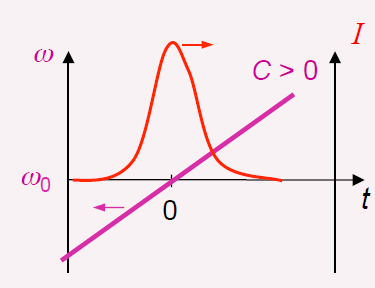
\includegraphics[scale=0.4]{ch1/image35}
	\captionof{figure}{ }
	\end{wrapfigure}
	La fréquence instantanée $\delta \omega$ à l'instant $t$ (contenu spectral à cet instant dans une
	fenêtre temporelle) évolue avec le temps. Si l'on "écoute" une impulsion passer on commencera
	dans le grave et la fréquence montera jusqu'à l'aiguë. Ici comme nous parlons spectralement, 
 	on commencera dans le rouge puis de plus en plus bleu. On appelle ça le \textbf{chirp}
 	(prononcer "tcheurp", comme le "tchip tchip des oiseaux (variation du son continue).\\
 	
 	\cadre{Un pulse est dit \textit{chirped} ($C\neq0$) si sa fréquence instantannée change avec
 	le temps.}\ \\
 	 	
 	Lorsque $b\neq0$, la phase temporelle est quadratique et décrite par le chirp $C$ : un $C>0$
 	signifie une augmentation linéaire de la fréquence instantanée. Pour $C=0$, on se situe à la
 	limite de Fourier. Si la phase est quadratique, un $\delta \omega$ commence négatif, il augmente,
 	passe au centre par la fréquence de la porteuse et puis continue à augmenter. Ici, le temps 
 	"négatif" signifie "arriver avant". \\
 	
 	Étudions la \textbf{propagation} ($z\neq0$). L'impulsion va acquérir une phase spectrale 
 	quadratique (la phase change, mais \textbf{reste} quadratique)
 	\begin{equation}
 	\tilde A(z,\omega ) = \tilde A(0,\omega )\exp ( - j[\frac{{{\beta _2}}}{2}{\omega ^2} + \frac{{{\beta _3}}}{6}{\omega ^3}]z)
 	\end{equation}
 	Le pulse pour $z\neq0 (\beta_3=0)$ est caractérisé par
 	\begin{equation}
 	b({z_1}) = {b_{z = 0}} + \frac{1}{2}{\beta _2}{z_1}
 	\qquad\text{ ou }\qquad
 	C({z_1}) = {C_{z = 0}} + {\beta _2}{z_1}W_0^2
 	\end{equation}
	Voyons comment le chirp change la durée de l'impulsion en évaluant le rapport
	\begin{equation}
	\frac{{{T_1}}}{{{T_{in}}}} = {\left[ {\frac{{1 + 4{b^2}W_0^4}}{{1 + 4b_{z = 0}^2W_0^4}}}
	 \right]^{1/2}} = {\left[ {\frac{{1 + C_{z = {z_1}}^2}}{{1 + C_{z = 0}^2}}} \right]^{1/2}}
	\end{equation}
	où $T_1 = HW\ 1/e$ est l'intensité au point $z=z_1$	et où $T_{in} = HW\ 1/e$ est l'intensité
	au point $z=0$. La largeur du pulse change lorsqu'il se propage ! \danger\ $C$ et $b$ ne sont
	pas toujours des fonctions croissantes avec la position car dépend du signe de $\beta_1$ et
	$z_1$.\\
	
	\begin{wrapfigure}[5]{l}{6cm}
	\vspace{-8mm}
	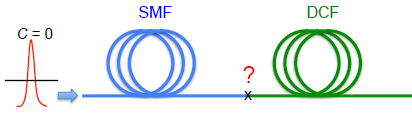
\includegraphics[scale=0.5]{ch1/image36}
	\captionof{figure}{ }
	\end{wrapfigure}
	Calculons l'évolution du pulse dans la configuration ci-contre. Initialement, nous avons un
	pulse à la limite de Fourier (phase plate, $C=0$). Après propagation dans la $SMF$, 
	l'impulsion est plus large. Pour une $DCF$, le \textit{slide 95} nous apprend que la phase
	temporelle doit être une parabole. Il va falloir "redresser" la phase avec le $DCF$ en prenant
	un $\beta_2$ de signe opposé à la $SMF$ : $C$ va se mettre à diminuer (en valeur absolue) et
	tendre progressivement vers zéro, en espérant revenir à l'impulsion du début. Ceci est 
	"semblable" avec la convergence d'un faisceau gaussien à travers une lentille.\\
	
		\begin{wrapfigure}[7]{r}{6cm}
	\vspace{-5mm}
	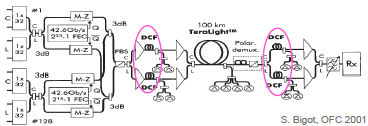
\includegraphics[scale=0.6]{ch1/image37}
	\captionof{figure}{ }
	\end{wrapfigure}
	Sur le montage (cf. schéma ci-contre), nous voyons avant et après la fibre des tronçons de 
	fibre à compensation de dispersion (DCF) (en deux parties pour limiter les effets 
	non-linéaires). Calculons la longueur de $DCF$ nécessaire pour contrecarrer la dispersion 
	dans la fibre \textit{TeraLight}. Les donnes sont les suivantes
	\begin{itemize}
	\item[$\bullet$] $L^{SMF}$ = 100km
	\item[$\bullet$] D$^{SMF}$ = 8 ps/(nm.km)
	\item[$\bullet$] D$^{DCF}$ = -50 ps/(nm.km)		
	\end{itemize}
	On cherche donc $L^{DCF}$. Sachant que $b({z_1}) = {b_{z = 0}} + \frac{1}{2}{\beta _2}{z_1}$, 
	on trouve
	\begin{equation}
	b(z=0)=0,\qquad  b(z=L^{SMF}) = \frac{1}{2} \beta_2^{SMF}.L^{SMF}
	\end{equation}
	\begin{equation}
	b(z=L^{SMF}+L^{DCF}) = \frac{1}{2} \beta_2^{SMF}.L^{SMF}+\frac{1}{2} \beta_2^{DCF}.L^{DCF}
	\end{equation}
	Pour ne pas avoir d'étalement, il faut que $ b(z=L^{SMF}+L^{DCF})=0$. La condition pour ne pas
	en avoir est donnée par 
	\begin{equation}
	\sum_j \beta_2^j L_ j = 0\qquad\Leftrightarrow\qquad\sum_j L_jD_j=0
	\end{equation}
	Il faut donc que $D^{DCF} = \left|\frac{D^{SMF}}{D^{DCF}} \right|L^{SMF} = 800/50= 16\text{ km}$.
	

	\subsubsection{Ordre de dispersion supérieur}
	\begin{wrapfigure}[5]{l}{5cm}
	\vspace{-7mm}
	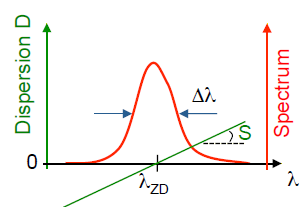
\includegraphics[scale=0.5]{ch1/image38}
	\captionof{figure}{ }
	\end{wrapfigure}
	On se rappelle que nous avions pour une fibre $B < \frac{1}{{\left| D \right|L\Delta \lambda }}$
	et pour plusieurs $B < \frac{1}{{\left| {\sum\nolimits_j {{L_j}{D_j}} } \right|\Delta \lambda }}$.
	Dès lors, si $D=0$ ou $\sum\limits_j {{D_j}{L_j}}  = 0$, $B$ pourrait être arbitrairement grand?
	Non, $BL$ reste limité par les effets dispersifs d'ordre supérieurs. Ces effets sont caractérisés
	par la \textbf{pente de dispersion} $S$\\
	
	\cadre{\textbf{Pente de dispersion $S$}\begin{equation}
	S = \frac{{{\rm{d}}D}}{{{\rm{d}}\lambda }} = {\left( {\frac{{2\pi c}}{{{\lambda ^2}}}} \right)^2}{\beta _3} + \frac{{4\pi c}}{{{\lambda ^3}}}{\beta _2}
	\end{equation}}\ \\
	
	En première approximation, lorsque $D=0$ il faut le remplacer par $S\Delta \lambda$ de sorte à 
	écrire
	\begin{equation}
	BL < \frac{1}{{\left| S \right|\Delta {\lambda ^2}}}
	\end{equation}
	où on voit apparaître un carré ! Au troisième ordre ($\beta_3$), la fonction est de type cubique :
	les pentes sont identique à gauche et à droite. Cela signifie que toutes les fréquences vont
	être décalées vers le même côté : tout se décale. On observe également des oscillations. En effet,
	certaines fréquences sont peu décalées et il en résulta un phénomène de battements.\\
	
	Dans les systèmes de multiplexage en longueur d'onde, la pente de dispersion est importante. 
	En effet, avec les DSF on peut seulement compenser la dispersion pour une seule longueur d'onde
	\begin{equation}
	D(\lambda ) = {S_0}(\lambda  - {\lambda _{ZD}})
	\end{equation}
	Comme pour la plupart des fibres $S>0$, on ne peut compenser la dispersion que pour un seul 
	channel. On peut travailler avec des fibres où $S$ est faible (fibre à pente réduite) ou des
	fibres où $S<0$ (fibre à inversion de dispersion).
	
	\subsubsection{Limitation du bit rate}
	\begin{wrapfigure}[7]{l}{6cm}
	\vspace{-5mm}
	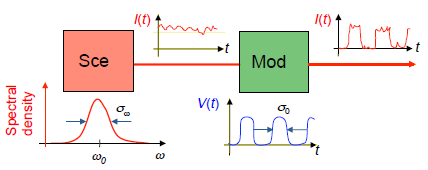
\includegraphics[scale=0.5]{ch1/image39}
	\captionof{figure}{ }
	\end{wrapfigure}
	Les effets dispersifs (vitesse de propagation différente en fonction de la longueur d'onde)
	causent	un élargissement de la taille du pulse qui peut limiter le \textit{bit rate}. La
	largeur spectrale à deux origines
	\begin{enumerate}
	\item La largeur spectrale finie de la source ($\sigma_w$)
	\item La forme temporelle (modulation) et la durée ($\sigma_0$)
	\end{enumerate}\ \\
	
	Nous allons considérer la propagation d'un pulse gaussien de longueur temporelle $\sigma_0$
	avec un spectre gaussien de longueur $\sigma_w$ pour \textbf{la source}. Rappelons que
	\begin{equation}
	{\sigma _t} \equiv \sqrt {\left\langle {{t^2}} \right\rangle  - {{\left\langle t \right\rangle }
	^2}} 
	\end{equation}
	où $\left(\langle t^m\rangle \equiv \int_{-\infty}^\infty t^m |A(t)|^2dt\right)/\left(\int_{-\infty}^\infty	 |A(t)|^2dt\right)$. On en tire
	\begin{equation}
	\frac{{{\sigma _t}^2}}{{\sigma _0^2}} = {\left( {1 + \frac{{C{\beta _2}L}}{{2\sigma _0^2}}} \right)^2} + (1 + V_\omega ^2){\left( {\frac{{{\beta _2}L}}{{2\sigma _0^2}}} \right)^2} + \frac{1}{2}{(1 + {C^2} + V_\omega ^2)^2}{\left( {\frac{{{\beta _3}L}}{{4\sigma _0^3}}} \right)^2}
	\end{equation}
	où $V_\omega \equiv 2\sigma_\omega\sigma_0$ et $C$ est pré-chirp du pulse. \\
	
	On peut calculer le \textit{bit rate} maximum en considérant que la largeur temporelle du 
	pulse doit être inférieure à $1/4$ du \textit{bit slot}\footnote{Le pulse gaussien a alors
	90\% de son énergie dans le bit slot}
	\begin{equation}
	\sigma_t < T_B/4 = \frac{1}{4B}
	\end{equation}
	Les \textit{slides 105} et \textit{106} donnent des exemples de calcul pour le produit $BL$ 
	(\textbf{à lire}).
	
	
	\subsection{Biréfringence et dispersion du mode de polarisation}
	La dispersion augmente les interférences inter-symbole, limitant le produit $BL$. Il y a 
	plusieurs mécanismes de dispersion
	\begin{description}
	\item[Dispersion modale] chaque mode se propage à sa propre vitesse de groupe
	\item[Dispersion chromatique] chaque fréquence se propage à sa propre vitesse de groupe
	\item[Dispersion de mode de polarisation] chaque état de polarisation principal se propage à
	sa propre vitesse de groupe
	\end{description}\ \\
	
	Les effets de polarisation dans les fibres n'affectent pas que l'\textbf{état de polarisation
	de sortie} mais il diminue aussi les \textbf{performances} du système de transmission (limitation
	du débit, la polarisation dans une fibre étant aléatoire).
	
	\subsubsection{Polarisation dans une fibre monomode}
	Considérons une fibre monomode où seul $LP_{01}$ se propage. Sous l'approximation du guidage
	faible, on trouve (dans le cœur), nous avons pour $LP_{01}$ ($N=1, q=1$) :
	\begin{equation}
	\left\{\begin{array}{ll}
	{E_z} &=\DS A{{J}_1}(\frac{{u.r}}{a}).\sin (\theta ).\exp (j[\omega t - \beta z])\\
	{E_r} &\DS= A( - j\beta \frac{a}{u}){{J}_0}(\frac{{u.r}}{a}).\sin (\theta ).\exp (j[\omega t - \beta z])\\
	{E_\theta } &\DS= A( - j\beta \frac{a}{u}){{J}_0}(\frac{{u.r}}{a}).\cos (\theta ).\exp (j[\omega t - \beta z])
	\end{array}\right.
	\end{equation}
	Dans un milieu massif, le champ électrique est orthogonal à la direction de propagation. Ce 
	n'est pas tout à fait le cas dans une fibre optique où la composante $z$ est non-nulle
	\begin{equation}
	|E_r| \approx |E_\theta| \approx \beta\frac{a}{u}|E_z|
	\end{equation}
	Cependant, comme
	\begin{equation}
	\beta \frac{a}{u} = \frac{{\beta .a}}{{\sigma .a}} = \frac{\beta }{{\sqrt {k_0^2{n_1}^2 - {\beta ^2}} }} = \frac{1}{{\sqrt {k_0^2{n_1}^2/{\beta ^2} - 1} }} \gg 1
	\end{equation}
	On peut dire que
	\begin{equation}
	{E_r}{^2} + {E_\theta }{^2} \gg {E_z}
	\end{equation}
	
	Pour les fibres à guidage faible, on a donc $\vec{E}\perp\vec{H}$ et $|E_z|/|\vec E|\ll 1$ soit
	presque des ondes $TEM$. Les \textbf{états de polarisation} (SOP) du mode $LP_{01}$ dans une
	fibre peut être décrit par un formalisme basé sur les \textbf{ondes planes dans le vide}. Nous
	allons faire un rappel sur la polarisation des ondes EM.	
	
	
	\subsubsection{État de polarisation (SOP) d'une onde EM}
	Les interactions lumière-matière se font via l'interaction de $\vec{E}$. Les \textbf{états de
	polarisation} correspondent à la trajectoire temporelle de la pointe du vecteur $\vec{E}$ (pour une
	position donnée)
	\begin{equation}
	\vec{E} = E_x\vec{1_x}+E_y\vec{1_y}
	\end{equation}
	où ${E_x} = {{\rm{E}}_{x0}}\cos (\omega t + {\varphi _x})$ et ${E_y} = {{\rm{E}}_{y0}}\cos (\omega
	 t + {\varphi _y})$ avec $E_{x0}$ et $E_{y0}$ les amplitudes de champ et $\varphi_x, \varphi_y$
	 les phases des champs. En éliminant $t$ et en posant $\Delta\varphi = \varphi_y-\varphi_x$ :
	 \begin{equation}
	 {[\frac{{{E_x}}}{{{{\rm{E}}_{x0}}}}]^2} + {[\frac{{{E_y}}}{{{{\rm{E}}_{y0}}}}]^2} -
	  2\frac{{{E_x}}}{{{{\rm{E}}_{x0}}}}\frac{{{E_y}}}{{{{\rm{E}}_{y0}}}}\cos (\Delta \varphi ) =
	   {\sin ^2}(\Delta \varphi )
	 \end{equation}
\newpage

	\begin{wrapfigure}[9]{l}{4cm}
%	\vspace{-5mm}
	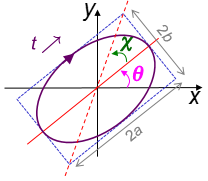
\includegraphics[scale=0.65]{ch1/image40}
	\captionof{figure}{ }
	\end{wrapfigure}
	 En toute généralité, l'état de polarisation d'une onde
	monochromatique polarisée est une \textbf{ellipse} dans le plan orthogonal à la propagation. 
	La forme de la trajectoire (et donc le SOP) est caractérisée par \textbf{deux} paramètres $\theta$
	(l'angle azimutal) et $\chi$ (définissant l'ellipticité) en plus de la direction
	\begin{equation}
	e \equiv \tan (\chi ) =  \pm \frac{b}{a}
	\end{equation}
	où $\pm =$ droite/gauche. Deux exemples sont donnés au \textit{slide 110}.
	
	
	\subsubsection{Propagation d'onde et évolution du SOP}
	La différence de phase $\Delta\varphi$ peut évoluer avec la distance de propagation. Selon le
	milieu, le SOP initial peut être \textbf{maintenu} ou \textbf{modifié} de façon déterministe ou
	aléatoire (fibre optique, difficile à prédire). Il existe quatre évolution de SOP
	\begin{enumerate}
	\item \textbf{Milieu isotope}\\
	La propagation est la même pour tous les états de polarisation : $\Delta \varphi_{prop}=0$, le
	SOP est maintenu.
	\item \textbf{Milieu linéaire biréfringent}\\
	Dans un tel milieu, il existe \textbf{deux direction perpendiculaires} dans lesquels deux états
	de \textbf{polarisation linéaire} qui se propagent resteront inchangés. Ce sont les axes 
	(principaux) du milieu. Ici nous avons
	\begin{equation}
	{E_x} = {{\rm{E}}_{x0}}\exp (j[\omega t - {\beta _x}z + {\varphi _{x0}}]),\qquad\qquad
	{E_y} = {{\rm{E}}_{y0}}\exp (j[\omega t - {\beta _y}z + {\varphi _{y0}}])
	\end{equation}
	avec les constantes de propagations le long des axes $x$ et $y$ (axes principaux). Dans ce cas-ci,
	$\Delta\varphi_{prop} = -(\beta_y-\beta_x)z$ : la différence de phase change linéairement avec
	 $z$. Le fait de faire une boucle dans le fibre optique introduit de la biréfringence.
	
	\item \textbf{Milieu à activité optique}\\
	Un SOP linéaire subit une rotation. Un SOP circulaire, rien ne change. Cette propriété vient du 
	déphasage entre les polarisations circulaires gauche et droite.
	
	\item \textbf{Matériau aléatoirement biréfringent}\\
	Le SOP de sortie n'est pas prévisible, c'est aléatoire : observé dans les fibres optiques 
	standard !	
	\end{enumerate}
	
	\subsubsection{Représentation mathématique d'un état de polarisation (SOP)}
	Il existe deux formalisme différent pour représenter un SOP : \textsc{Jones} (sur $E_x,E_y, 
	\varphi_x, \varphi_y$) et \textsc{Stokes} ($\theta, \chi$).\\
	
	\textsc{Formalisme de Jones}\\
		\begin{wrapfigure}[7]{r}{3cm}
	\vspace{-5mm}
	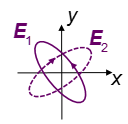
\includegraphics[scale=0.8]{ch1/image41}
	\captionof{figure}{ }
	\end{wrapfigure}
	Le SOP est représenté par un vecteur de Jones $V$ (représentation en phaseur)
	\begin{equation}
	V \equiv \left( {\begin{array}{*{20}{c}}
{{{\rm{E}}_{x0}}\exp (j{\varphi _x})}\\
{{{\rm{E}}_{y0}}\exp (j{\varphi _y})}
\end{array}} \right)
	\end{equation}
	où ${\left\| {\;V\;} \right\|^2} = {{\rm{E}}_{x0}}^2 + {{\rm{E}}_{y0}}^2$. On normalise 
	habituellement $V$ et $E_{x0}, E_{y0}, \Delta \varphi$ (le SOP) peuvent être déduit de $V$. Les
	deux états de polarisation $V_1$, $V_2$ sont orthogonaux
	\begin{equation}
	V_1^\dag {V_2} = V_2^\dag {V_1} = 0\qquad\Leftrightarrow\qquad {\theta _1} - {\theta _2} = \pi /
	2\,\,\,\& \,\,\,{\chi _1} =  - {\chi _2}
	\end{equation}
	Des exemples de vecteur de Jones sont donnés au \textit{slide 114}.\\
	
	Dans un milieu linéaire, la polarisation de sortie dépend linéairement de celle en entée
	\begin{equation}
	{V_{OUT}} = \underbrace{\left( {\begin{array}{*{20}{c}}
A&B\\
C&D
\end{array}} \right)}_{J}.{V_{IN}}
	\end{equation}
	où $J$ est la \textbf{matrice de Jones} (la matrice de transfert entre le SOP d'entrée et de sortie)
	qui est généralement complexe. Par conservation de l'énergie
	\begin{equation}
	{J^\dag }J = J{J^\dag } = 1
	\end{equation}
	Le formalisme traite aisément la propagation à travers un système optique constitué de différents
	milieux
	\begin{equation}
	{V_{OUT}} = {J_n}...{J_3}{J_2}{J_1}{V_{IN}}
	\end{equation}
	\begin{center}
		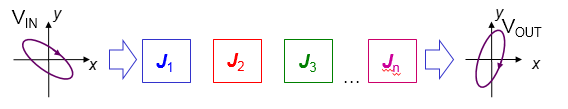
\includegraphics[scale=0.74]{ch1/image42}
	\captionof{figure}{ }
	\end{center}
	La matrice de Jones possède \textbf{deux vecteurs propres orthogonaux}
	\begin{equation}
	{B_{OUT}} = J.{B_{IN}} = \lambda {B_{IN}}
	\end{equation}
	Ces modes propres ($B_{in}$) voient leur polarisation inchangée par propagation entre 
	l'entrée et à la sortie (mais pas "entre" les deux). Dans un matériau biréfringent linéaire, 
	les vecteurs propres sont les axes de polarisation. Le \textit{slide 116} donne des exemples
	de matrices de Jones\footnote{Lire les notes de ce slide, intéressant}.\\
	
	
	Le \textit{formalisme de Jones} est puissant et facile à utiliser (il conserve même la phase
	absolue, ce qui est perdu avec le formalisme de \textit{Stokes}). Cependant, il n'est pas
	toujours le plus adéquat car il ne fonctionne pas lorsque l'onde est non monocrhomatique, la
	fréquence dépend de la biréfringence du milieu, la lumière est partiellement polarisée et la
	polarisation non linéaire. \\
	
	Un autre aspect non-négligeable est la difficulté de mesurer une différence de phase
	$\Delta \varphi$. Avec une référence c'est "facile" mais si on est seulement en présence
	d'un champ c'est presque impossible à déterminer indirectement. On va alors faire des mesures
	indirectes et c'est le principe de fonctionnement du \textit{formalisme de Stokes}.\\
\newpage	
	\textsc{Formalisme de Stokes}\\
	Ce formalisme est lié à la différence de puissance (intensité) entre les états de polarisation
	orthogonaux. Les paramètres sont les suivants
	
	\begin{description}
	\item[Intensité totale] 
	\begin{equation}
	{S_0} = E_{x0}^2 + E_{y0}^2
	\end{equation}
	\item[Différence d'intensité entre les polarisations linéaires $x$ \textit{et} $y$]
	\begin{equation}
	{S_1} = E_{x0}^2 - E_{y0}^2
	\end{equation}
	\item[Différence d'intensité entre les polarisations linéaires à $+45^\circ$ et $++135^\circ$]	
	\begin{equation}
	{S_2} = 2E_{x0}^{}E_{y0}^{}\cos (\Delta \varphi )
	\end{equation}
	\item[Différence d'intensité entre les polarisation circulaire droite et gauche]
	\begin{equation}
	{S_3} = 2E_{x0}^{}E_{y0}^{}\sin (\Delta \varphi )
	\end{equation}
	\end{description}
	On définit le vecteur de Stokes comme
	\begin{equation}
	S \equiv {({S_0}\,{S_1}\,{S_2}\,{S_3})^T}
	\end{equation}
	Que l'on normalise souvent tel que $s \equiv {(1\,\,{s_1}\,{s_2}\,{s_3})^T}$. Lorsque la
	lumière est totalement polarisée, on a
	\begin{equation}
	s_1^2 + s_2^2 + s_3^2 = 1
	\end{equation}
	Si l'on pouvait mesurer de façon instantanée l'évolution du champ, celle-ci serait
	toujours polarisée mais cette mesure n'est pas toujours accessible. Par exemple avec une 
	impulsion polarisée horizontalement et l'autre verticalement (qui se suivent), si le détecteur
	à un temps de capture plus long que le passage des deux impulsions, il "verra" une onde
	totalement dépolarisée  alors que ce n'est pas le cas. Dans ce cas, on aura une lumière
	partiellement polarisée et donc
	\begin{equation}
	s_1^2 + s_2^2 + s_3^2 < 1
	\end{equation}

	\begin{wrapfigure}[7]{l}{10.75cm}
	\vspace{-5mm}
	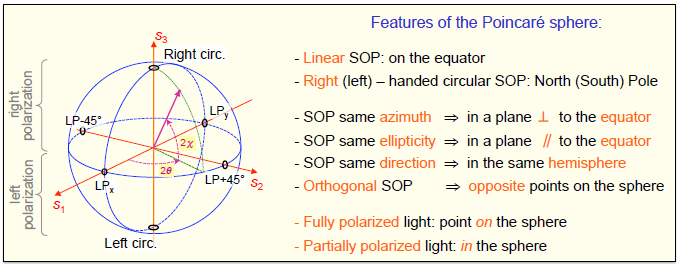
\includegraphics[scale=0.6]{ch1/image43}
	\captionof{figure}{ }
	\end{wrapfigure}
	Dans le cas général d'une polarisation elliptique (totalement polarisé), le vecteur de Stokes
	s'écrit
	\begin{equation}
	s = \left( {\begin{array}{*{20}{c}}
1\\
{\cos (2\theta )\cos (2\chi )}\\
{\sin (2\theta )\cos (2\chi )}\\
{\sin (2\chi )}
\end{array}} \right)
	\end{equation}\ \\
	
	Ceci suggère qu'un SOP totalement polarisé est représenté par un point \textbf{sur} la sphère
	de Poincaré (alors qu'il sera "dans" la sphère lorsque la polarisation est partielle). En effet,
	$s_1, s_2$ et $s_3$ sont les composantes d'un vecteur unitaire de coordonnées sphériques
	$(2\theta, 2\chi)$.\\
	
	\newpage
	\exemple{\textsc{Propagation dans un milieu biréfringent linéaire}\ \\
	Soit $\beta_x, \beta_y$ les constantes de propagation pour l'axe $x$ (axe rapide) et $y$ 
	(axe lent) : $\beta_x<\beta_y$ et un SOP linéaire à $45^\circ$. En supposant un milieu 
	biréfringent linéaire avec $q=0$, posons $\delta = (\beta_y-\beta_x)z$ et 
	$\varphi = (\beta_y+\beta_x)z$.\\
	
	Dans le formalisme de \textbf{Jones}, la polarisation d'entrée étant linéaire il n'y a pas 
	de déphasage entre les deux composantes d'amplitudes ici égales
	\begin{equation}
	{V_{in}} = \frac{1}{{\sqrt 2 }}\left( {\begin{array}{*{20}{c}}
1\\
1
\end{array}} \right)
	\end{equation}
	La matrice de Jones du système est
	\begin{equation}
	J = \left( {\begin{array}{*{20}{c}}
{\cos (\delta /2) + j\sin (\delta /2)}&0\\
0&{\cos (\delta /2) - j\sin (\delta /2)}
\end{array}} \right){e^{ - j\varphi /2}}
	\end{equation}
	On en tire
	\begin{equation}
	V(z) = \frac{1}{{\sqrt 2 }}\left( {\begin{array}{*{20}{c}}
{\cos (\delta /2) + j\sin (\delta /2)}\\
{\cos (\delta /2) - j\sin (\delta /2)}
\end{array}} \right){e^{ - j\varphi /2}}
	\end{equation}
	La forme générale du vecteur de Stokes étant donné par
	\begin{equation}
	V = \exp (j\xi )\left( {\begin{array}{*{20}{c}}
{\cos (\theta )\cos (\chi ) - j\sin (\theta )\sin (\chi )}\\
{\sin (\theta )\cos (\chi ) + j\cos (\theta )\sin (\chi )}
\end{array}} \right)
	\end{equation}
	Par identification, on en tire que
	\begin{equation}
	\left\{\begin{array}{ll}
	\theta &= \pi/4\\
	\chi  &=  - \delta /2 =  - \Delta \beta z/2
	\end{array}\right.
	\end{equation}
	L'orientation de l'ellipse ne va \textbf{pas} changer, mais l'ellipticité va évoluer 
	en fonction de $z$. \\
	
	En partant d'une polarisation initiale $LP, +45^\circ$ on va se balader dans un plan coupant la
	sphère de Poincaré, plan contenant les axes $S_2$ et $S_3$.
	\begin{center}
		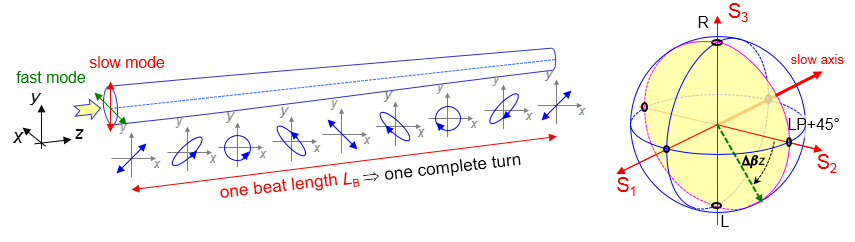
\includegraphics[scale=0.6]{ch1/image44}
	\captionof{figure}{ }
	\end{center}
	On va parler de \textit{longueur de battement} la longueur $z$ d'une "période, correspondant à 
	la rotation sur la sphère de Poincaré dans la direction de l'axe lent (angle positif).}
	
	
	
	\newpage
	Ce résultat peut être généralisé : \\
	
	\cadre{\textbf{Propagation à travers un élément à biréfringence elliptique}\\
	La transformation est équivalente à une rotation anti-horraire autour du SOP du mode lent 
	(flèche verte)avec un taux de rotation égal à $\Delta \beta$
	\begin{center}
		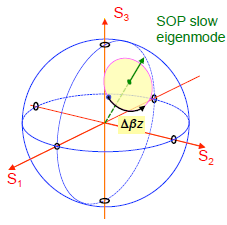
\includegraphics[scale=0.6]{ch1/image45}
	\captionof{figure}{ }
	\end{center}	
	}\ \\
	
	Une rotation complète correspond à une longueur de propagation égale à la longueur de battement
	\begin{equation}
	{L_B} = \frac{{2\pi }}{{\Delta \beta }} = \frac{{2\pi }}{{{\beta _{slow}} - {\beta _{fast}}}}
	\end{equation}
	où $\Delta\beta = \beta_{slow}-\beta_{fast}$.





\subsubsection{Origine de la biréfringence dans les fibres}
Dans les fibres optiques, le biréfringence vient d'une brisure de symétrie d'un cœur et 
gaine parfaitement circulaire avec un indice de réfraction localement isotropique. Elle a plusieurs
origines physiques
\begin{enumerate}
\item \textit{Cœur non circulaire : brisure de symétrie.}\\
Si le cœur n'est pas symétrique, appliquer les $CL$ pour un mode horizontal ne donnera pas la même
chose que pour un mode vertical. 
\begin{equation}
n_x\neq n_y\qquad\Leftrightarrow\qquad \beta_x\neq \beta_y
\end{equation}
	\begin{center}
		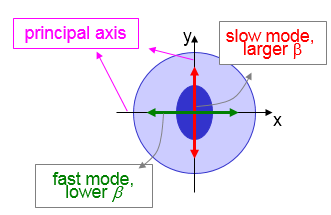
\includegraphics[scale=0.6]{ch1/image46}
	\captionof{figure}{ }
	\end{center}	
On peut s'attendre à être dans un milieu de biréfringence linéaire. Le résidu typique de biréfringence
est de $\Delta n = {n_y} - {n_x} \approx {10^{ - 7}}$ (celui-ci vaut $\approx 10^{-7}$ dans une fibre
à maintient de polarisation).

\item \textit{Présence de contraintes.}\\
L'effet élasto-optique fait en sorte que la propagation modifie $n$. En refroidissement la fibre
de façon non-homogène on peut introduire des contraintes internes induisant une variation de $n$
via l'effet élasto-optique. On peut aussi introduire des contraintes externes (en pressant par exemple
sur la fibre). 

\item \textit{Plier la fibre : introduit des contraintes dans la fibre.}\\
En pliant, la moitié de la fibre est en compression et l'autre en élongation : la contrainte est 
non uniforme et cela mène à une biréfringence linéaire avec comme axe lent (plus grand $\beta$, champ
plus confiné) l'axe parallèle à l'axe
de courbure
	\begin{center}
		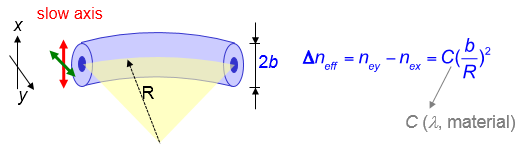
\includegraphics[scale=0.65]{ch1/image47}
	\captionof{figure}{$R$ est le rayon de courbure et $2b$ le diamètre extérieur de la fibre.}
	\end{center}	
	
\item \textit{Torsion}.\\
Introduit de la biréfringence circulaire : les polarisations circulaires gauches et droites sont 
maintenues mais leurs constantes de propagation sont différentes. La variation de phase entre les
deux est donnée par
\begin{equation}
\Delta \varphi  = {\beta _{CR}} - {\beta _{LR}}L \approx 1.146\;K\;L
\end{equation}

\item \textit{Présence d'un champ électrique transverse.}
\item \textit{Présence d'un champ magnétique longitudinal.}
\end{enumerate}\ \\

Les sources principales de biréfringence dans une fibre sont les quatre premières. Certaines sont
constantes avec le temps, d'autres évoluent à \textbf{cause des conditions environnementales}. 
L'amplitude et l'orientation de la biréfringence le long d'une fibre est donc inconnue (sauf pour
les fibres à maintient de polarisation). 

\subsubsection{Fibre à maintient de polarisation}
	\begin{wrapfigure}[8]{l}{8cm}
	\vspace{-5mm}
	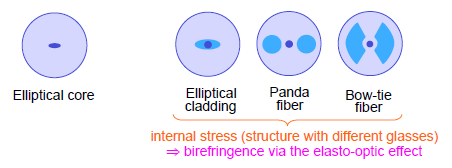
\includegraphics[scale=0.64]{ch1/image48}
	\captionof{figure}{ }
	\end{wrapfigure}
Parfois, il est très important de maintenir le SOP (surtout en télécommunication). Dans les SMF, 
la polarisation est très sensible aux conditions environnementales : le SOP de sortie est instable
et à priori inconnu. On utilisera alors des \textbf{fibres à maintient de polarisation} PMF. Celles-ci
sont caractérisée par une \textbf{grande} biréfringence linéaire obtenue en introduisant une forte
asymétrie circulaire dans la section de la fibre.


\subsubsection{Dispersion des modes de polarisation (PMD)}
La biréfringence affecte l'état de polarisation, mais elle cause également l'\textbf{élargissement}
de pulses : \textit{polarization mode dispersion}. La forme du pulse sera ainsi modifiée car 
les modes propres n'ont pas seulement des vitesses de phases différentes, mais également des
vitesses de groupes différentes. Il existe deux régimes.\\

\textsc{1. Régime intrinsèque $PMD_i$}\\
\begin{itemize}
\item[$\bullet$] La biréfringence n'a qu'une valeur sur toute la longueur de la fibre,
\item[$\bullet$] Les modes propres sont des SOPs linéaires,
\item[$\bullet$] \textbf{Pas} de couplage de puissance entre ces modes.
\end{itemize}
Le temps de vol est donné par
\begin{equation}
\tau = \frac{L}{v_g} =  L \frac{\partial \beta}{\partial \omega} = L 
\frac{\partial}{\partial \omega}\left(\frac{2\pi}{\lambda_0}n_{eff}(\lambda_0)\right)
\end{equation}
Sachant que
\begin{equation}
\dfrac{\partial}{\partial\omega} = -\frac{\lambda_0^2}{2\pi c}\dfrac{\partial}{\partial\lambda_0}
\end{equation}
On en tire
\begin{equation}
\tau = -\frac{L 2\pi}{2\pi c}\lambda_0^2\left[ \frac{-1}{\lambda_0}n_{eff} + \frac{1}{\lambda_0}
\lambda_0\frac{\partial}{\partial\lambda_0}n_{eff}\right]
\end{equation}
Après simplification, on trouve
\begin{equation}
{\tau _{gx}} = \frac{z}{c}(n_{eff}^x - \lambda \frac{{dn_{eff}^x}}{{d\lambda }}),\qquad\qquad
{\tau _{gy}} = \frac{z}{c}(n_{eff}^y - \lambda \frac{{dn_{eff}^y}}{{d\lambda }})
\end{equation}
Soit
\begin{equation}
\Delta {\tau _p} = {\tau _{gy}} - {\tau _{gx}} = \frac{z}{c}(\Delta n_{eff}^{} - \lambda \frac{{d\Delta n_{eff}^{}}}{{d\lambda }}) = \frac{z}{c}\Delta {N_{eff}}
\end{equation}

\begin{center}
	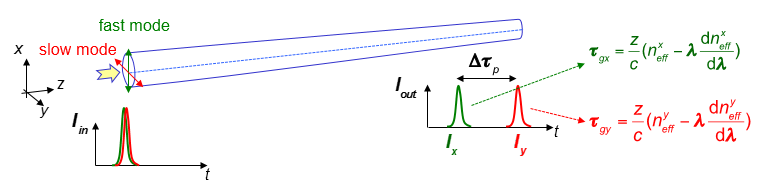
\includegraphics[scale=0.64]{ch1/image49}
	\captionof{figure}{ }
\end{center}

Le délai de groupe différentiel (DGD, la différence de temps de vol) est la différence de délai entre
deux pulses orthogonaux situés le long des axes principaux de la fibre. On peut donc interpréter
le DGD comme un étalement du pulse, limitant le produit $BL$. Dans le cas intrinsèque, on va 
définir un coefficient lié à ce mécanisme de dispersion de mode de polarisation
\begin{equation}
PM{D_i} \buildrel \Delta \over = \frac{{\Delta {\tau _p}}}{z} = \frac{{\Delta N_{eff}^{}}}{c}
\end{equation}
C'est le \textbf{coefficient de dispersion de mode de polarisation (intrinsèque)}, qui s'exprime
en \textbf{ps/km} !\\

La $PMD_i$ se mesure facilement dans le domaine spectral. La différence de phase entre deux modes
polarisés selon les axes principaux est
\begin{equation}
\Delta \varphi  = \Delta \beta L = \frac{\omega }{c}\Delta {n_{eff}}(\omega )L
\end{equation}
Cette différence de phase peut augmenter si $L$ augmente ou si la fréquence de la porteuse $\omega$
augmente. Dans les deux cas, l'évolution est périodique dans le sens où elle "dessine" un cercle
sur la sphère de Poincaré.

\newpage

	\begin{wrapfigure}[7]{r}{3cm}
%	\vspace{-5mm}
	\includegraphics[scale=0.5]{ch1/image50}
	\captionof{figure}{ }
	\end{wrapfigure}
Expérimentalement, on peut facilement faire varier $\omega$. On va s'arranger pour que $\Delta \omega$
soit tel que le SOP de sortie soit le même que le SOP d'entrée (on change la fréquence jusqu'à 
retrouver le même état de polarisation). Ceci est possible que si $\Delta\varphi$ augmente de $2\pi$. 
Avec la précédente formule
\begin{equation}
\Delta \varphi  + 2\pi  = [\frac{{\omega  + \Delta \omega }}{c}\Delta {n_{eff}}(\omega ) + \frac{\omega }{c}\Delta \omega \frac{d}{{d\omega }}\Delta {n_{eff}}(\omega )]L
\end{equation}
On peut faire apparaître l'expression du $PMD_i$
\begin{equation}
2\pi  = \Delta \omega [\frac{{\Delta {n_{eff}}}}{c} + \frac{\omega }{c}\frac{d}{{d\omega }}\Delta {n_{eff}}]L = \underbrace{PM{D_i}\;L}_{\Delta\tau_p}\;\Delta \omega 
\end{equation}
Finalement
\begin{equation}
\frac{{2\pi }}{{\;\Delta \omega }} = \frac{1}{{\;\Delta \nu }} = \Delta {\tau _p}
\end{equation}
On en tire que la DGD est simplement reliée au changement en fréquence nécessaire pour prendre
prendre le SOP de sortie à travers un cycle complet.\\





\textsc{2. Régime couplé}\footnote{Pas génial, bien relire \textit{slides} !}\\
Le long de la fibre, l'orientation des axes principaux et de la biréfringence ne \textbf{peut pas} 
être considérée comme constant sur l'entièreté de la fibre. Un tel résultat peut être obtenu via
la concaténation de petites fibres possédant toute une biréfringence linéaire différente.
\begin{center}
	\includegraphics[scale=0.75]{ch1/image51}
	\captionof{figure}{ }
\end{center}
L'évolution du SOP est alors difficile à prédire : une polarisation linéaire initialement le long
d'un axe principal peut être couplé à une polarisation orthogonale (projection du champ dans les
axes propres au moment de la jointure). A cause du couplage entre les polarisation à chaque
"jointure", le PMD couplé est moins limitant que l'intrinsèque : c'est pourquoi on conseille de souder
 les fibres avec une orientation aléatoire. \\

 
 On peut écrire, dans le formalisme de Jones
 \begin{equation}
 {V_{OUT}} = {J_{biref}}({q_n},{\delta _n})\;...\;{J_{biref}}({q_2},{\delta _2}){J_{biref}}({q_1},
 {\delta _1}){V_{IN}}
 \end{equation}
 Si la "biréfringence map" peut être totalement caractérisée ($\delta_i, q_i$), le SOP de sortie peut
 être précisément connu pour chaque entre
 \begin{equation}
 {V_{OUT}}(\omega ) = {J_{span}}(\omega ){V_{IN}}
 \end{equation}\ \\
 \newpage
 	Appelons un \textit{span}  la concaténation des fibres de biréfringence éventuellement 
	différentes.\\

	 Même pour des spans complexes, il existe \textbf{deux états de polarisation d'entrée}
	(PPS, Principal Polarization State) à $\omega$ fixé
	\begin{itemize} 
	\item[$\bullet$] Ces deux états sont orthogonaux
	\item[$\bullet$] Ils ne changent pas avec des petites variation de fréquences (ordre 1)
	\item[$\bullet$] Le PPS de sortie est orthogonaux et différent du PPS d'entrée
	\end{itemize}\ 
	
	Par définition, pour les (deux) PPS de sortie
	\begin{equation}
	\mathop {\lim }\limits_{\Delta \omega  \to 0} \frac{{{p_{out}}(\omega  + \Delta \omega ) -
	 {p_{out}}(\omega )}}{{\Delta \omega }} = 0
	\end{equation}

		\begin{wrapfigure}[9]{l}{7cm}
%	\vspace{-5mm}
	\includegraphics[scale=0.4]{ch1/image52}
	\captionof{figure}{ }
	\end{wrapfigure}
	Comme le PPS de sortie ne dépend pas de la fréquence (au premier ordre), on peut définir un
	délai de groupe pour les deux PPS orthogonaux. Il n'y aura alors qu'un changement de la phase
	globale du vecteur de Jones du PPS de sortie avec la fréquence. \textbf{Un pulse initial 
	tel que SOP = PPS d'entrée ne propage sans distosion} (au premier ordre). Un délai de groupe
	$\tau_g = \partial\tilde{\varphi}/\partial\omega$ peut être défini entre les deux PPSs.	\\
	
	Si par contre le SOP d'entrée est différent des PPSs, il y aura élargissement du signal à cause
	de la DGD entre les deux PPSs. Dans les vrai fibre, la "biréfringence map" évolue à cause de
	l'environnement : DGD change aléatoirement avec le temps ! La seule approche cohérente pour
	le PMD est \textbf{statistique}.\\
	
	En effectuant des mesures à différentes moments de la journée, on trouve une distribution 
	approximativement proche d'une distribution Maxwellienne. Dans ce régime, on a donc
	\begin{equation}
	\left\langle {\Delta {\tau _{pc}}} \right\rangle  \propto \sqrt L 
	\end{equation}
	Le coefficient de PMD dans le régime couplé aura alors les unités de \textbf{ps.km$^{-1/2}$}
	\begin{equation}
	PM{D_c} \buildrel \Delta \over = \frac{{\left\langle {\Delta {\tau _{pc}}} \right\rangle }}{{\sqrt
	 L }}
	\end{equation}
	En présence de $N$ sections de fibres différentes
	\begin{equation}
	PM{D_{tot}}\sqrt {{L_{tot}}}  = \sqrt {PMD_1^2{L_1} + PMD_2^2{L_2} + ... + PMD_N^2{L_N}} 
	\end{equation}\ \\
	
	En pratique, PMD est signifiant lorsque DGD est supérieur à 30\% du temps bit
	\begin{equation}
	DGD_{max} = 0.3T_B
	\end{equation}
	Le prolbème est que $\Delta \tau_{pc}$ est aléatoire et peut être bien plus grand que la valeur 
	moyenne. On veut alors que la probabilité de dépasser la valoir maximale soit inférieure à
	$4\times 10^{-5}$ ce qui est vrai (selon la distribution Maxwellienne) si
	\begin{equation}
	DG{D_{max}} = 3\left\langle { {\Delta \tau _{pc}}} \right\rangle 
	\end{equation}
	Lorsque la dispersion chromatique est compensée, le PMD est le paramètre limitant.